%%%%%%%%%%%%%%%%%%%%%%%%%%%%%%%%%%%%%%%%%%%%%%%%%%%%%%%%%%%%%%%%%%%%%%%%%%%%%%%%%%
% The new ACM style from 2017!
% - http://sensys.acm.org/2017/resources/documents/HowTo.pdf
% - http://www.acm.org/publications/proceedings-template
% - http://www.acm.org/binaries/content/assets/publications/consolidated-tex-template/acmart.pdf
%%%%%%%%%%%%%%%%%%%%%%%%%%%%%%%%%%%%%%%%%%%%%%%%%%%%%%%%%%%%%%%%%%%%%%%%%%%%%%%%%%
\documentclass[10pt,sigconf,letterpaper,anonymous]{acmart}
%\documentclass[10pt,sigconf,letterpaper]{acmart}% new ACM style 2017 + anonymous


% BELOW 3 LINES FOR REVIEW VERSION ONLY (REMOVE FOR CAMERA READY)
\settopmatter{printacmref=false} % Removes citation information below abstract
\renewcommand\footnotetextcopyrightpermission[1]{} % removes footnote with conference info
\pagestyle{plain} % removes running headers

%%%%%%%%%%%%%%%%%%%%%%%%%%%%%%%%%%%%%%%%%%%%%%%%%%%%%%%%%%%%%%%%%%%%%%%%%%%%%%%%

\usepackage{subfigure}                  % For subfigure
\usepackage{multirow}                   % For multirow table
\usepackage{enumitem}                   % For [leftmargin=*] option in itemize
\usepackage{balance}                    % For balanced columns on the last page

\newcommand{\jw}[1]{{\textcolor{green!55!blue}{\it JW: #1}}}
\newcommand{\jp}[1]{{\textcolor{orange}{\textit{JP: #1}}}}
\newcommand{\jk}[1]{{\textcolor{blue}{\textit{JK: #1}}}}
\newcommand{\wj}[1]{{\textcolor{magenta}{\textit{WJ: #1}}}}
\newcommand{\raj}[1]{{\textcolor{cyan}{\textit{RB: #1}}}}
\newcommand{\todo}[1]{{\textcolor{red}{\textbf{TODO: #1}}}}
\newcommand{\rev}[1]{{\textcolor{black}{#1}}}

\newcommand\spar[1]{\vspace{1ex}\noindent{\bf #1}}

\newcommand{\tworow}[1]{\multirow{2}{*}{#1}}
\newcommand{\twocol}[1]{\multicolumn{2}{|c|}{#1}}

\newcommand{\system}{{LoGR}}                     % old style
\newcommand{\sysit}{\textit{\system}}
\newcommand{\myname}{LoGR}                     % old style
\newcommand{\myit}{\textit{\myname}}

\newcommand{\mlo}{{Magic Leap One}}

\newcommand{\fig}{Figure~}
\newcommand{\figs}{Figures~}
\graphicspath{{./figure/}}

%%%%%%%%%%%%%%%%%%%%%%%%%%%%%%%%%%%%%%%%%%%%%%%%%%%%%%%%%%%%%%%%%%%%%%%%%%%%%%%%%%

% formatting hack, iff needed ... only at the last moment
%\setlength{\textfloatsep}{12pt}        % space between figure and text
%\setlength{\floatsep}{9pt}             % space between figure and figure
%\setlength{\subfigbottomskip}{3pt}     % space at bottom of subfigure
%\setlength{\subfigtopskip}{2pt}        % space at top of subfigure
%\setlength{\subfigcapskip}{-1pt}

%%%%%%%%%%%%%%%%%%%%%%%%%%%%%%%%%%%%%%%%%%%%%%%%%%%%%%%%%%%%%%%%%%%%%%%%%%%%%%%%%%

\copyrightyear{2018}


% Copyright
%\setcopyright{acmcopyright}     % if you give the rights to ACM ==> DEFAULT
\setcopyright{none}             % none
%\acmDOI{...}                    % DOI - Insert your DOI below...
%\acmISBN{...}                   % ISBN - Insert your conference/workshop's ISBN below...
%\acmYear{2018}                  % Insert Publication year
%\copyrightyear{2018}            % Insert Copyright year (typically the same as above)
%\acmPrice{15.00}
%\acmConference[Short Name]{Long Name}{dates}{venue}

%%%%%%%%%%%%%%%%%%%%%%%%%%%%%%%%%%%%%%%%%%%%%%%%%%%%%%%%%%%%%%%%%%%%%%%%%%%%%%%%%%

\begin{document}

%\title[short title]{long long title}
\title[LoGR]
    %{\huge LpGL: Low-power Graphics Library using Sensor-based User Perception
    %    for Untethered AR Head Mounted Displays}
    {\huge {\myit}: Low-power Graphics Library \textit{for} Mobile AR Headsets}
    %{\huge C'Mon! You Can't See That Anyway - \\A Low-power Graphics Library \textit{for} Mobile AR Headsets}
    %{\huge SaveME: Saving Energy Usage on Mobile AR Headsets}

%\titlenote{titlenote stuff}
%\subtitle{subtitle stuff}
%\subtitlenote{subtitle note stuff}

%%%%%%%%%%%%%%%%%%%%%%%%%%%%%%%%%%%%%%%%%%%%%%%%%%%%%%%%%%%%%%%%%%%%%%%%%%%%%%%%%%

\author{Jaewon Choi}
    %\authornote{you can put authornote stuff here}
    %\orcid{1234-5678-9012}
    \affiliation{%
     \institution{Ajou Univerisity}
%     \department{Department of Computer Engineering}  
      %\country{Republic of Korea} 
    }
\email{jainersoer@ajou.ac.kr}

\author{HyeonJung Park}
    \affiliation{%
     \institution{Ajou University}
%     \department{Department of Computer Engineering}
      %\country{Republic of Korea} 
    }
\email{jhikm1003@ajou.ac.kr}

\author{Jeongyeup Paek}
    %\authornote{this guy has a son and a daughter}
    \affiliation{%
     \institution{Chung-Ang University}
%     \department{School of Computer Science and Engineering}
      %\country{Republic of Korea} 
    }
\email{jpaek@cau.ac.kr}

\author{Rajesh Krishna Balan}
    %\authornote{this guy has a son and a daughter}
    \affiliation{%
     \institution{Singapore Management University}
%     \department{School of Information Systems}
      %\country{Republic of Korea} 
    }
\email{rajesh@smu.edu.sg}

\author{JeongGil Ko}
    \affiliation{%
     \institution{Ajou Univerisity}
%     \department{Department of Computer Engineering}
      %\country{Republic of Korea} 
    }
\email{jgko@ajou.ac.kr}

%%%%%%%%%%%%%%%%%%%%%%%%%%%%%%%%%%%%%%%%%%%%%%%%%%%%%%%%%%%%%%%%%%%%%%%%%%%%%%%%%%

% The default list of authors is too long for headers
\renewcommand{\shortauthors}{Jaewon Choi et al.}

%%%%%%%%%%%%%%%%%%%%%%%%%%%%%%%%%%%%%%%%%%%%%%%%%%%%%%%%%%%%%%%%%%%%%%%%%%%%%%%%%%

% Abstract must precede \maketitle
\begin{abstract}
%%%%%%%%%%%%%%%%%%%%%%%%%%%%%%%%% 80 CHAR %%%%%%%%%%%%%%%%%%%%%%%%%%%%%%%%%%%%%%
%
%
% Recent advances in augmented reality (AR) technology are attracting 
% various emerging industrial and everyday life applications.
% %
% However, resource limitations of untethered HMDs, in particular, the energy 
% constraint of battery-powered devices, can limit the scope of potential applications.
% %
% Hence, a common approach is to lower the visual quality, which however
% trades-off user perceived experience for energy efficiency.
% %
% A key requirement for such applications, then, is to enhance the 
% energy efficiency %of untethered HMD devices
% while minimizing the sacrifice in user experience.
%
%
% In this work, we present {\myit}, an OpenGL API compatible 
%
We present {\myit}, an OpenGL API compatible \emph{Low-power Graphics Library}
for energy efficient AR headset applications.
%
%Prior to presenting the design of {\myit}, 
We first characterize power consumption patterns of a state of the art 
AR headset, Magic Leap One, and empirically show that its internal GPU is 
the most impactful controllable energy factor.
%
Based on preliminary studies, we design {\myit} so that it uses the 
device's gaze/head orientation information
and geometry data to infer user perception information, 
intercepts application-level graphics API calls, 
and uses frame rate control, mesh simplification, and culling techniques
to enhance energy efficiency of AR headsets without detriment of user experience.
%
%
% We evaluate {\myit} using a prototype implementation on Microsoft HoloLens.
%
Results from a comprehensive set of controlled in-lab experiments and an 
IRB-approved user study with 25 participants
%
%show that {\myit} can reduce the HoloLens' energy usage by $\sim$25\% 
show that {\myit} reduces up to $\sim$22\% of total power while adding only 46$\mu$sec of latency per object with close to no loss in subjective user 
experience.
%
%
%%%%%%%%%%%%%%%%%%%%%%%%%%%%%%%%% 80 CHAR %%%%%%%%%%%%%%%%%%%%%%%%%%%%%%%%%%%%%%



\begin{comment}


We present {\myit}, an OpenGL API compatible Low-power Graphics Library
for energy efficient AR headset applications.
%
%Prior to presenting the design of {\myit}, 
We first characterize power consumption patterns of a state of the art 
AR headset, Magic Leap One, and empirically show that its internal GPU is 
the most impactful controllable energy factor.
%
Based on preliminary studies, we design {\myit} so that it uses the 
device's gaze/head orientation %information
and geometry data to infer user perception information, 
intercepts application-level graphics API calls, 
and uses frame rate control, mesh simplification, and culling techniques
to enhance energy efficiency of AR headsets without detriment of user experience.
%
%
% We evaluate {\myit} using a prototype implementation on Microsoft HoloLens.
%
Results from a comprehensive set of controlled in-lab experiments and a user study with 25 participants
%
%show that {\myit} can reduce the HoloLens' energy usage by $\sim$25\% 
show that {\myit} reduces up to $\sim$22\% of total power (0.8~hr increase from 2.7~hr lifetime) while adding only 46$\mu$sec of latency per object with no loss in subjective user 
experience.
%
%
%%%%%%%%%%%%%%%%%%%%%%%%%%%%%%%%% 80 CHAR %%%%%%%%%%%%%%%%%%%%%%%%%%%%%%%%%%%%%%


\end{comment}

\end{abstract}

%
% The code below should be generated by the tool at
% http://dl.acm.org/ccs.cfm
% Please copy and paste the code instead of the example below. 
%
% \begin{CCSXML}
% <ccs2012>
%     <concept>
%         <concept_id>10003033.10003106.10003112.10003238</concept_id>
%         <concept_desc>Networks~Sensor networks</concept_desc>
%         <concept_significance>500</concept_significance>
%     </concept>
%     <concept>
%         <concept_id>10010405.10010444.10010447</concept_id>
%         <concept_desc>Applied computing~Health care information systems</concept_desc>
%         <concept_significance>500</concept_significance>
%     </concept>
%     % <concept>
%     %     <concept_id>10002951.10003227.10003241.10003244</concept_id>
%     %     <concept_desc>Information systems~Data analytics</concept_desc>
%     %     <concept_significance>300</concept_significance>
%     % </concept>
% </ccs2012>
% \end{CCSXML}

% \ccsdesc[500]{Networks~Sensor networks}
% \ccsdesc[500]{Applied computing~Health care information systems}
% \ccsdesc[300]{Information systems~Data analytics}


% We no longer use \terms command
%\keywords{Augmented Reality, Energy Efficiency, Head Mounted Display, OpenGL
%}

\maketitle

%%%%%%%%%%%%%%%%%%%%%%%%%%%%%%%%%%%%%%%%%%%%%%%%%%%%%%%%%%%%%%%%%%%%%%%%%%%%%%%%%%

\vspace{-2ex}
\section{Introduction}
\label{sec:intro}

%%%%%%%%%%%%%%%%%%%%%%%%%%%%%%%%%%%%%%%%%%%%%%%%%%%%%%%%%%%%%%%%%%%%%%%%%%%%%%%%
% Background

Augmented reality (AR) applications are starting to be used in various  
real-world application domains, ranging from industrial engineering, 
clinical services, field repairs, to lifestyle 
management~\cite{Wang2016,pokemongo,ikeaplace,augmedix,evalARVRTraining}.
%
To support these real-world on-site use cases, mobile untethered AR headsets 
such as the Microsoft HoloLens~\cite{hololens}, 
Google Glass~\cite{googleglass}, and Magic Leap One~\cite{magicleapone} 
are now commercially available. 
%
Typically, these ``untethered'' mobile headsets differ from tethered devices 
in that they are fully self-contained and have the CPU, GPU, and 
networking capabilities to run full AR applications without access to 
more powerful computing devices. % nearby.
%
Thus, they enable AR applications to be used in any location and environment,
allowing a much richer set of viable use cases.



%%%%%%%%%%%%%%%%%%%%%%%%%%%%%%%%%%%%%%%%%%%%%%%%%%%%%%%%%%%%%%%%%%%%%%%%%%%%%%%%
% Problem statement

% Challenge 1: AR devices are suffering energy/battery issue

The challenge is that untethered AR headsets are \emph{resource constrained} 
\textit{mobile} computing platforms.
%
In particular, they are intentionally designed to be lightweight and have 
minimal heat buildup. % to avoid hurting the user while being head mounted.
%
As such, untethered AR headsets have limited battery capacity 
(to reduce weight), and use less powerful CPU and GPUs 
(to reduce power usage and heat), 
%
which can limit their usefulness % of untethered AR devices
in many real-world use cases. 
%
For example, the {\mlo} has only 2 to 3 hr usage time~\cite{magicleapone}, which may not be
sufficient for use cases that do not allow for convenient access to recharging.


%This is in particular due to the energy constraints, an inherent limitation 
%as a battery-powered mobile device.
%
%The main consumers of energy in AR devices are the CPU, GPU, display and 
%wireless communication modules. 
% used for implementing realistic scenes and interactions.
%
%such as all-day life or serious medical surgery applications.
%
%In other words, battery lifetime is important not only for improving user 
%experience, but also for widening application scope.
%
%Thus, lengthening the battery lifetime of HMDs is an important problem to solve.


%%%%%%%%%%%%%%%%%%%%%%%%%%%%%%%%%%%%%%%%%%%%%%%%%%%%%%%%%%%%%%%%%%%%%%%%%%%%%%%%
%
% Challenge 2: considerations for reducing energy consumption on a mobile device


%\raj{To Fix: 1) make it clearer why this is a mobile and not plain graphics solutions. 2) make it clear that this works on closed devices. thus we are limited in what we can do which impact our choices. but we do it well. DONE!!!}

A key approach to maximize battery lifetime on mobile devices involves reducing 
the fidelity of applications or hardware components on the mobile device. 
However, these trade-offs must be carefully managed to avoid sacrificing 
user experience.
%
In this paper, we present {\myit}, a low-power graphics library that 
automatically adjusts the resource usage of AR applications to reduce 
power consumption significantly with minimal loss of user experience\footnote{A video of {\myit} in use is available at \url{http://is.gd/logr\_mobisys}}.
%
{\myit} requires no changes to application source code as it abstracts and
hides all energy efficiency considerations in lower layers that are invisible 
to user applications (Section~\ref{sec:system}).
%
This is achieved by re-writing, re-ordering, and selectively executing
user API requests in the underlying {\myit} layer based on user perception.

Specifically, {\myit} uses gaze/head orientation and 3D object geometry data to obtain
user perception information, and combines three main techniques to reduce power
consumption of applications while preserving usability;
%
\begin{enumerate}[leftmargin=*]

    \item Dynamics score calculation for frame rate scaling,
    
%    \item Mesh simplification for reducing the projected object complexity, and
     \item Mesh simplification for reducing object complexity, and
    
    \item Culling for reducing draw calls counts to minimize power 
    consumption without impacting user experience. 

\end{enumerate}
%
These techniques operate based on the key user and mobility information 
provided by the AR device to enact its final power savings configuration.
%
In particular, {\myit} uses (a) dynamic head and eye tracking of where the user
is looking at currently, 
%with b) dynamic tracking of ambient conditions, 
and (b) the selected power usage profile (off, normal, high, etc.) to achieve an
output that saves a high amount of power with minimal usability impact. 

\begin{figure}
    \centering
    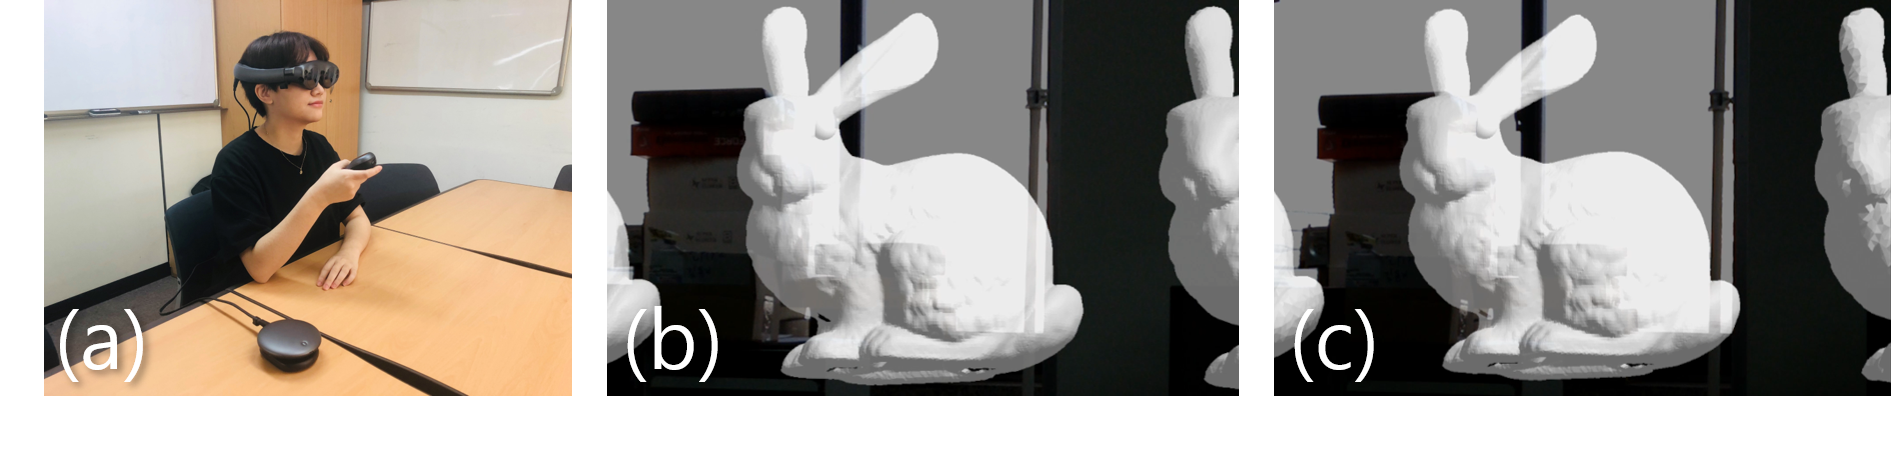
\includegraphics[width=1\linewidth]{comparison}
    \vspace{-4ex}
    \caption{Study participant with {\mlo} (a) with scenes observed from baseline (b) and {\myit} (c).}
    \label{fig:comparison}
\end{figure}



The primary goal of this work is to provide a solution that would work across 
various AR devices -- regardless of their manufacturer and software setup.
%
As such, we focused on adapting software and device aspects only those that
are accessible across all AR devices we surveyed. 
%(Section~\ref{sec:background})
%for survey results).
%
%From our survey, w
We found that most AR devices use proprietary software that
provides limited access to the hardware of the AR device. 
%
In particular, the head, eye, hand, and inertial tracking subsystems of these
AR devices were not easily modifiable -- you could read their values easily
but there was no access to change their settings to, for example, 
implement a duty cycling scheme.
%
However, all the surveyed devices provided OpenGL graphics libraries that
allowed good access to the rendering subsystems. Thus, to be as device 
independent as possible, we focused our efforts primarily on the rendering 
subsystems (while using inputs from the sensing components to drive our
adaptation) and defer adaptation of other energy-consuming components to 
future work -- or such a time where easy access to these subsystems becomes 
possible.

For this reason, {\myit} provides an OpenGL ES 3.0 compatible graphics API 
wrapper that is used to modify the application's OpenGL API calls to output 
a modified command set that reduces system-level power consumption.
%
This allows {\myit} to be highly device- and application- independent, 
and as transparent as possible to both applications and users.
%
Note: users may see a different output when {\myit} is enabled (especially if 
more aggressive power saving modes are selected) 
-- however this new output is still sufficient and acceptable for the task 
the user is performing and minimally disturbing within the user's core focal angle.
%
\fig\ref{fig:comparison} shows a sample scene presented using the baseline and {\myit}.


%%%%%%%%%%%%%%%%%%%%%%%%%%%%%%%%%%%%%%%%%%%%%%%%%%%%%%%%%%%%%%%%%%%%%%%%%%%%%%%%

We implemented {\myit} on the {\mlo}~\cite{magicleapone} (Section~\ref{sec:inlab})
and conducted an extensive set of in-lab experiments to evaluate its
system-level performance under various configurations.
%
In addition, we performed an IRB-approved user study with 25 student participants
to understand the usability impact of {\myit} (Section~\ref{sec:userstudies}).
%(c.f., \fig\ref{}).
%
%For this we conduct an Institutional Review Board (IRB) approved pilot %study
%with 25 university students.
%
Our results from in-lab experiments and the user study show that {\myit}
reduces the power usage by as much as $\sim$22\% 
with only marginal ($\sim$46$\mu$sec) added latency per displayed 
object on a frame and minimal loss in subjective user experience levels.
%
This power reduction translates to achieving 3.9 hours of continuous system lifetime, compared to 3.0 hours when using the baseline graphics library directly.
%
Furthermore, our experiments show that {\myit} results in similar or lower device 
temperature with the baseline approach while achieving higher frame rates.
%(Section~\ref{sec:eval}).

The major contributions of this paper are as follows:

\begin{itemize}[leftmargin=*]

    \item Detailed power measurements of {\mlo}, a commercial AR device, to inform and guide the design of {\myit}.

    \item Combining mobility features with rendering techniques to allow {\myit} to reduce GPU and memory usage power costs in a scalable manner.

    \item Detailed in-lab power and device temperature measurements showing the efficacy of {\myit}.

    \item Results from a 25 participant user study showing that {\myit} does not impact usability, accuracy, or task times.

\end{itemize}



%%%%%%%%%%%%%%%%%%%%%%%%%%%%%%%%%%%%%%%%%%%%%%%%%%%%%%%%%%%%%%%%%%%%%%%%%%%%%%%%

% Specifically, this paper makes the following contributions.
% %
% \vspace{-0.5ex}
% \begin{itemize}[leftmargin=*]
% %
%     \item We perform in-depth analysis on energy consumption patterns of 
%         an untethered AR HMD platform. We show that object complexity, frame rate and 
%         the number of draw calls heavily affect AR HMD's energy usage.
%         (Sec.~\ref{sec:preliminary})
    
%     \item We present {\myit}, an OpenGL API compatible library for
%         enhancing AR HMD's energy efficiency.
%         It uses the gyroscope to infer user perception, and transparently
%         modifies graphics operations to be more energy efficient.
%         (Sec.~\ref{sec:system}).
    
%     \item We conduct a comprehensive set of in-lab experiments as well as pilot 
%         deployments at an ophthalmology department in a university hospital.
%         Results show that 
%         {\myit} effectively reduces the AR HMD's energy usage while
%         minimally affecting latency and user experience. 
%         (Sec.~\ref{sec:app} and~\ref{sec:eval})
        
% \end{itemize}

%%%%%%%%%%%%%%%%%%%%%%%%%%%%%%%%%%%%%%%%%%%%%%%%%%%%%%%%%%%%%%%%%%%%%%%%%%%%%%%%

% The remainder of this paper is structured as follows.
% %
% We first present a preliminary study on the energy usage of AR HMD platform in
% Section~\ref{sec:preliminary}, which motivates and guides our design of {\myit}.
% %
% We then describe the design and key ideas of {\myit} in Section~\ref{sec:system},
% and discuss the implementation issues in Section~\ref{sec:implementation}.
% %
% We evaluate our system in Section~\ref{sec:eval}, 
% discuss related work in Section~\ref{sec:related},
% and conclude the work in Section~\ref{sec:conclusion}.

%%%%%%%%%%%%%%%%%%%%%%%%%%%%%%%%%%%%%%%%%%%%%%%%%%%%%%%%%%%%%%%%%%%%%%%%%%%%%%%%


\section{Preliminary Study: AR Headsets}
%\section{Preliminary Study on AR Headset}
\label{sec:preliminary}

\subsection{Background}
\label{sec:background}
% \raj{moved from intro. will merge soon}

%

\begin{comment}

However, prior studies raise three questions that need to be answered
when designing an energy management scheme using perceptual information;
%
(1) What sources of information on human perception can we access?
(2) How can we recognize human perception using sensory data?, and
(3) What can we do to reduce energy usage?
%
Our approach is to address the energy efficiency problem on mobile HMDs
by answering each of these three questions.

\end{comment}

%%%%%%%%%%%%%%%%%%%%%%%%%%%%%%%%%%%%%%%%%%%%%%%%%%%%%%%%%%%%%%%%%%%%%%%%%%%%%%%%

In this work, we are developing power management solutions for untethered mobile AR headsets, and base our approach on two core characteristics of these types of headsets - (1) the variable scene sparsity, and (2) the ever changing user perception. A key difference of dedicated AR headsets is that, unlike virtual reality (VR) applications, and mobile phone-based AR applications, AR headsets \emph{do not need to render backgrounds}. In particular, VR or phone applications require the system to draw a virtual \textit{background}, and mobile AR applications need to overlay images captured from the video camera on the screen. However for AR headsets, the user directly observes ``reality'' through a translucent lens, and only the virtual objects (e.g. 3D models) are augmented on the scene with an empty background. As a result, the problem  scope of energy efficient object rendering is different from full-screen rendering systems. In addition, untethered headsets, unlike tethered devices, have to perform the computationally expensive rendering process \textit{on the mobile device itself} rather than on a nearby PC and simply displaying the content on the display.

Another key characteristic of mobile AR headsets is that they require 
some form of orientation or \emph{user perception} information. For example, devices such as the Hololens exploit gyroscope-based head orientation data and the {\mlo} offers both gyroscope and gaze tracking data. These sensors inform the device on what direction the user's visual attention is focused towards and what they are paying attention to. This is important as the device needs to understand where to focus its limited computational power on.

Finally, as stated in the introduction, most commercial untethered AR headsets are currently being released as ``closed'' platforms where a large amount of the software and sensors running the device is not accessible to third-party developers, making it difficult to access low level information and optimize system performance.
%
For example, the {\mlo} uses its Lumin OS~\cite{magicleapone}, which is a sandboxed platform that provides limited access to low level information -- thus limiting what third-party programs can do for performance enhancement. This is similar to the  HoloLens~\cite{hololens}, which uses the Universal Windows Platform (UWP)~\cite{uwp}. 
%
Naturally, this complicates the design and implementation of optimization
approaches for most (even experienced) developers and suggests 
the need for an underlying layer to optimize the energy usage
silently and obliviously to the application. Fortunately, in all cases, we found that AR devices all supported OpenGL. Thus, we chose to implement our performance improvements in the OpenGL layer as way of achieving cross-device compatibility -- albeit at the loss of access to sensors and information, such as the eye and gaze tracking hardware, not accessible through graphics library APIs.


%%%%%%%%%%%%%%%%%%%%%%%%%%%%%%%%%%%%%%%%%%%%%%%%%%%%%%%%%%%%%%%%%%%%%%%%%%%%%%%%


%%%%%%%%%%%%%%%%%%%%%%%%%%%%%%%%% 80 CHAR %%%%%%%%%%%%%%%%%%%%%%%%%%%%%%%%%%%%%%

% \begin{comment}

% Why did this preliminary studies: AR HMD is new environment so there are few 
% energy analysis reports.
% Unlike traditional smartphone and VR HMDs, most recent AR HMDs have different 
% hardware components.
% For example, 
% - Display:  traditional devices have LCD display, however Google glasses uses 
%             Prism projector, Microsoft HoloLens uses liquid crystal on silicon 
%             (LCoS) displays.
% Architecture: smartphones use mobile GPU and VR HMDs use desktop GPU
% - resources but Microsoft HoloLens use HPU(Holographic Processing Unit).
% It works not only as GPU, hardware level vision processing also.

% AR HMD's core components:

% \begin{itemize}
%     \item CPU: 4 core
%     \item HPU(Holographic Computing Unit): similar with GPU, but has small number of cores (24 cores)
%     \item Networking
%     \item display
% \end{itemize}

% Potentially affecting factors but limited:

% \begin{itemize}
%     \item Resolution: In graphics perspective, But we cannot control this.
%     \item Brightness: We did but it was not major. Usual mobile phone use HMD 
%         but HoloLens use liquid crystal on silicon (LCoS) displays.
%     \item Networking datarate: It affects some, but it is closed system. 
%         we cannot modify internal parameters or policy.
% \end{itemize}

% Controllable factors:

% \begin{itemize}
%     \item # of triangles
%     \item # of draw calls
%     \item frame rate
% \end{itemize}

% Correlations:

% \begin{itemize}
%     \item If # of triangles increases, # of draw calls effects more
%     \item If # of triangles increases, frame rate effects more
%     \item If # of draw calls increases, frame rate effects more
% \end{itemize}
 
% Results: frame rate matters and if we can decrease # of triangles and 
%     # of draw calls we make cost of frame rate cheaper.

% - \cite{Hwang:2017:RPO:3117811.3117841} introduce Y-space

% \end{comment}

%%%%%%%%%%%%%%%%%%%%%%%%%%%%%%%%% 80 CHAR %%%%%%%%%%%%%%%%%%%%%%%%%%%%%%%%%%%%%%

\subsection{Detailed Power Measurements}

We next performed a detailed study to understand the power usage characteristics of the {\mlo} commercial untethered AR headset. This is a representative of typical untethered AR headsets and consists of three core components: computation, 
display, and networking. Our goal was to identify the power consumption of each component under various workloads and use these results to focus our power conservation solutions. 

%These components cooperate to render/display images, and 
%exchange data as requested by the application.
%
%
The {\mlo} consists of two major (portable) components: the headset and 
the computation device. The headset contains a liquid crystal on silicon (LCoS) 
display, offering a fixed 1280x960 resolution, with a gaze tracking device and IMU sensors. The computational device, which is wired to the headset, contains an Nvidia Tegra X2 SoC with two Denver 2.0 64-bit cores and four ARM Cortex A57 64-bit core. It also contains an integrated Pascal-based GPU with 256 CUDA cores, with 8 GBs of RAM.  Finally, the computation device also contains a Murata 802.11 ac/b/g/n and Bluetooth 4.0 chipset.
%
We could not find any detailed breakdowns of recently-released untethered AR headsets' power consumption. Thus, this preliminary study is also a good reference for other researchers wanting to optimize power consumption of AR devices. To perform this preliminary study, we ran tasks that used different system configurations 
(e.g., object complexity, display configurations, and network data rate), and measured the power usage of each component using the {\mlo} developer interface. Unless explicitly specified, the frame rate for was set to 60 frames per second (fps), the default frame rate for {\mlo}.

%To better understand the impact of the ``controllable factors'' that affect energy 
%usage performance, we performed a set of experiments that measure the energy 
%consumption of a HoloLens. 
%%
%Specifically, by running simple applications with different configurations 
%(e.g., network data rate, display configurations and object complexity),
%for $\sim$10 minutes each, we measure the amount of energy used in units of 
%mWh/10minutes, as offered by the HoloLens' UWP API.
%%
%Also, unless explicitly mentioned otherwise, the frame rate is set to 60 frames
%per second (fps), the default frame rate for Microsoft HoloLens applications.
%%

\begin{figure}[t]
    \centering
    \vspace{-1ex}
    \subfigure[Total power consumption]{
        % \includegraphics[width=0.27\linewidth]{min_max_cropped}
        \label{fig:total-energy}
    }
    \hfill
    \subfigure[Per-component power consumption]{
        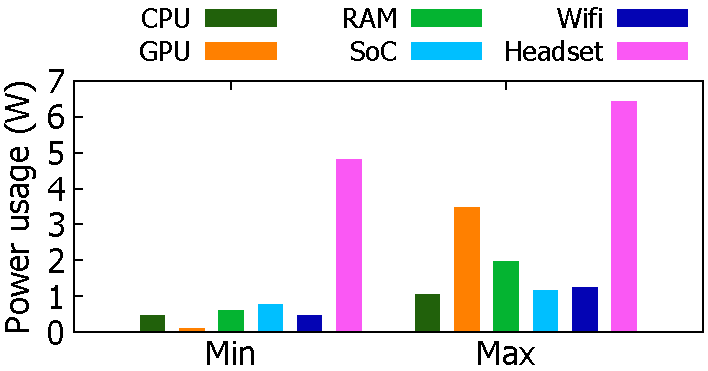
\includegraphics[width=0.62\linewidth]{min_max_component_cropped}
        \label{fig:component-energy}
    }
    \vspace{-2ex}
    \caption{Power usage breakdown for minimum and maximum performance cases on the \mlo.}
    \label{fig:minmax-energy}
\end{figure}





%%%%%%%%%%%%%%%%%%%%%%%%%%%%%%%%% 80 CHAR %%%%%%%%%%%%%%%%%%%%%%%%%%%%%%%%%%%%%%

\subsection{Minimum and Maximum Power Usage}

We first performed a simple experiment to measure the minimum and maximum power consumption on the \mlo. For the minimum case, after switching on the device, we displayed no content, the controller was not connected to the headset, and all computing and networking features were disabled except for the always-on baseline functionality. For measuring the maximum power usage, we set the device to render at maximum rate (1.0M polygons at 60 FPS), send packets at full line rate ($\sim$14 MB/s over UDP), and connected the controller to the headset via Bluetooth. \fig\ref{fig:minmax-energy} shows detailed power measurements for the two extreme cases. We observe that at the maximum, the power consumption increased by more than 110\% compared to the minimum case.
%
Furthermore, we notice that the headset, which includes sensors for gaze tracking, gyroscope, and the LCoS display, dominates the power usage. %Unfortunately, 
Even though the headset is consuming nearly 42\% of the total power usage when operating at maximum, unfortunately, like many commercially available AR headsets, the {\mlo} does not allow developers to control headset sensors' parameters (such as enforcing an energy-optimized duty cycling).

Fortunately, even without the headset, the computational units, including all the processors and networking interfaces, still consumes, compared to minimum case, as much as 6.5~W more and $\sim$58\% of the total system power. Thus, optimizing the power consumption of the computational unit can still result in significant power savings and increased usage time of the AR device. For example, we found that the {\mlo}, using its 36.7~Wh battery, could only run for about 2.4 hours at the maximum power usage configuration and for 5.1 hours with the minimum configuration.


\subsection{Graphics Rendering Components}

%\begin{figure}[t]
%    \centering
%    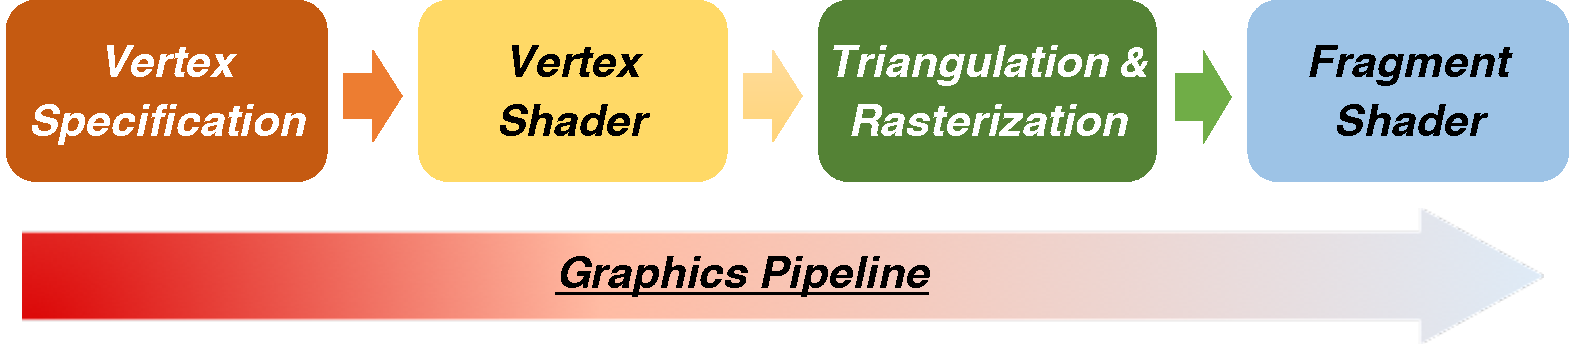
\includegraphics[width=0.9\linewidth]{RenderingPipeline-1}
%    %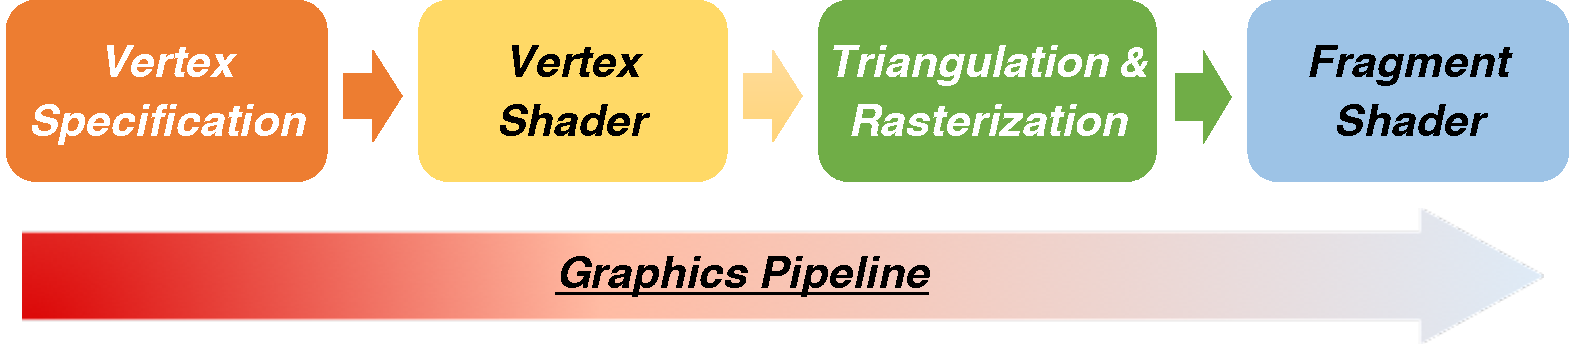
\includegraphics[width=\linewidth]{RenderingPipeline-2}
%    \vspace{-2ex}
%    \caption{Graphics pipeline for 3D object rendering.}
%    \label{fig:pipeline}
%\end{figure}

We first look into the impact the graphics components of the {\mlo} has on the overall power usage. A typical ``graphics pipeline'',
% (\fig\ref{fig:pipeline}), 
in this case for AR devices, consists of computationally heavy operations (e.g., matrix computation and rasterization), that use source information representing 3D objects (e.g. triangle and texture information) and output rendered 2D images. For seamless user experience, the rendering pipeline should run at 60 fps or higher. However, this high fps requires a large amount of computation, in turn, requires a lot of power usage.

Before measuring the power consumption of the graphics pipeline, we first explain how applications interact with the graphics rendering libraries. To render a specific geometry (e.g., 3D object), a typical application will need to send three types of information to the graphics API:  (1) vertices and their topology information, (2) transformation matrix of a model, and (3) command to draw the object (i.e., draw call).

%The geometry to be drawn is specified by the vertices list (that define the 3D mesh) along with the topology information listing how these vertices are connected. The transformation matrix translates, rotates, and scales the arbitrary vertices to achieve the final desired shape -- the graphics pipeline multiplies this matrix to each vertex. Finally a ``draw call'' is made to physically draw an object to the screen. 

%%%%%%%%%%%%%%%%%%%%%%%%%%%%%%%%% 80 CHAR %%%%%%%%%%%%%%%%%%%%%%%%%%%%%%%%%%%%%%



% On vertex shader stage, the computing units of GPU perform transformation 
% operations for every each vertex in parallel.
% After other geometric operations, for example Vertex Post-Processing, graphics
% pipeline triangulates vertices using topology information.
% Based on output, triangles, rest of pipeline rasterize it and executes 
% per-pixel operations to generate final 2D image for the screen.
% Through those facts we can get fundamental idea: The number of vertices to 
% be rendered determines the intensity of the rendering.


%%%%%%%%%%%%%%%%%%%%%%%%%%%%%%%%% 80 CHAR %%%%%%%%%%%%%%%%%%%%%%%%%%%%%%%%%%%%%%

\begin{figure}[t]
    \centering
    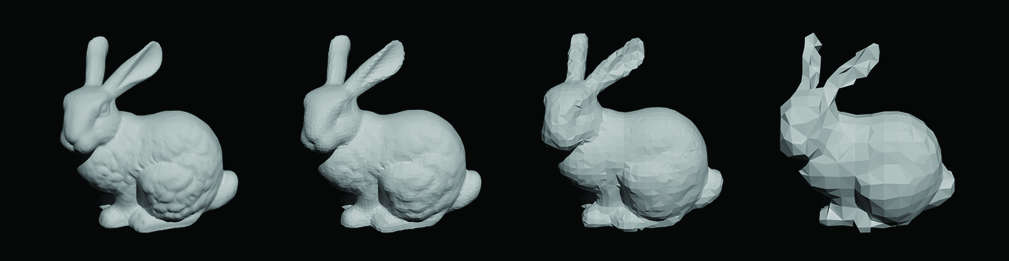
\includegraphics[width=0.9\linewidth]{stanfordBunnies}
    \caption{The Stanford Bunny~\cite{bunny} in four different resolutions, 
            with different number of triangles. 
            %Left shows the highest quality and the quality degrades towards the right.
            }
    \label{fig:bunny}
\end{figure}


\begin{figure}[t]
    \centering
    \vspace{-1ex}
    \subfigure[Total consumption]{
        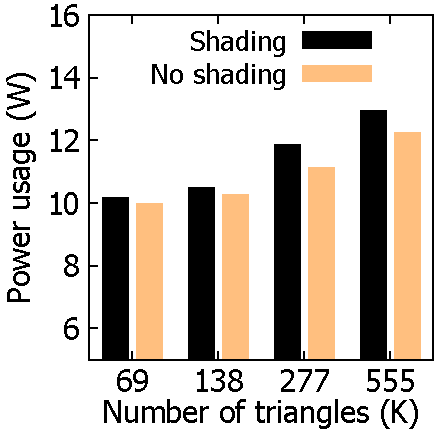
\includegraphics[width=0.45\linewidth]{complexity_cropped}
        \label{fig:complexity-total}
    }
    \hfill
    \subfigure[GPU and memory with shading]{
        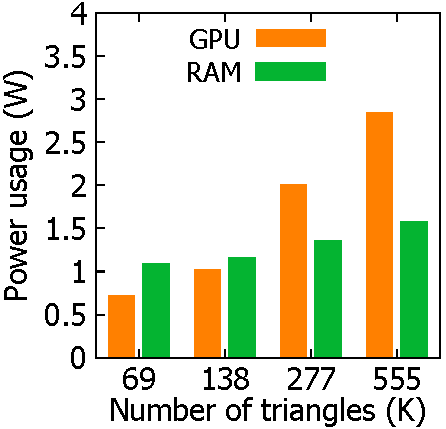
\includegraphics[width=0.45\linewidth]{triangles_gpu_ram_cropped}
        \label{fig:complexity-gpu}
    }
    \vspace{-2ex}
    \caption{Power consumption plots for varying object complexity (object triangle count).}
    \label{fig:complexity}
\end{figure}




%%%%%%%%%%%%%%%%%%%%%%%%%%%%%%%%% 80 CHAR %%%%%%%%%%%%%%%%%%%%%%%%%%%%%%%%%%%%%%

\spar{Number of vertices}:
%
To quantify the power consumption of different \emph{number of vertices},
we use the widely used Stanford Bunny model (\fig\ref{fig:bunny})~\cite{bunny} in four different resolutions. The left-most bunny in \fig\ref{fig:bunny} is
the full resolution object containing 69K triangles, with the subsequent 
bunnies containing 16K, 3.7K, and 900 triangles, respectively. Note: a triangle is a basic mesh object, comprised of multiple vertices, that is used to create the final 3D object -- the more triangles used, the more realistic and smoother the final object.

%To examine the performance of the intermediate cases, we also created bunnies 
%with $\sim$32K and $\sim$48K triangles; thus, test for a total of six different 
%object complexities. 

The power consumption results, in Figure~\ref{fig:complexity-total}, for rendering these four bunnies suggests that the {\mlo} consumes a fixed amount of power ($\sim$10~W) to render up to 138K triangles. Beyond this point, the 
power consumption starts to increase. We also observe that the shading process consumes a significant amount of power. Quantitatively, when increasing the object complexity from 69K to 555K triangles, we observed a 3.6~W (35\%) increase with shading enabled, and a 1.8~W (17\%) increase without shading. From 
\fig\ref{fig:complexity-gpu}, which plots the GPU and memory usage 
for different object complexities with shading, we observed that the power consumption increase is caused by increased GPU and memory usage -- with the GPU, by itself, consuming nearly 4x more power as the complexity increases. These results suggest that controlling the number of vertices in the object model (to reduce image complexity), can be an effective strategy in reducing the device's power usage.


%%%%%%%%%%%%%%%%%%%%%%%%%%%%%%%%% 80 CHAR %%%%%%%%%%%%%%%%%%%%%%%%%%%%%%%%%%%%%%

%\begin{figure}[t]
%    \centering
%    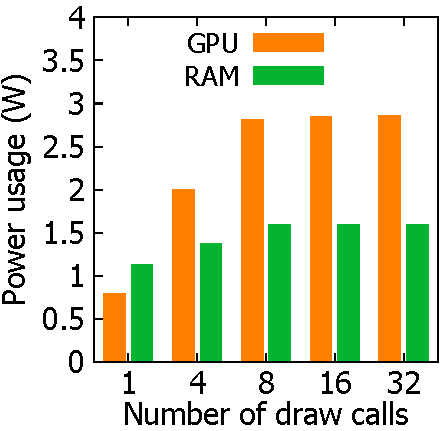
\includegraphics[width=0.8\linewidth]{drawCall_cropped}
%    \vspace{-2ex}
%    \caption{Energy consumption rate with varying number of draw calls 
%            (and thus objects) at 60 fps. }
%    \label{fig:drawCall}
%\end{figure}


\begin{figure}[t]
    \centering
    \vspace{-1ex}
    \subfigure[Total consumption]{
        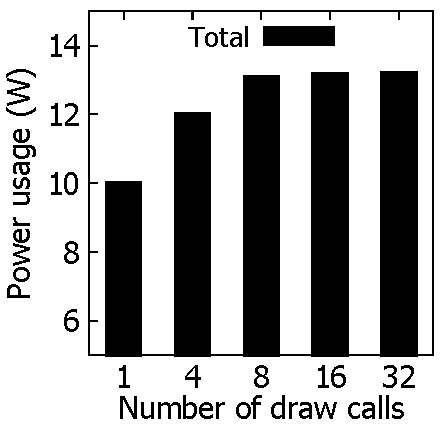
\includegraphics[width=0.45\linewidth]{drawCall_total_cropped}
        \label{fig:drawCall-total}
    }
    \subfigure[Power breakdown]{
        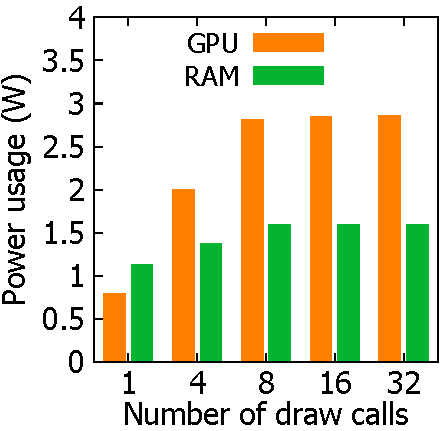
\includegraphics[width=0.45\linewidth]{drawCall_cropped}
        \label{fig:drawCall-gpu}
    }
    \vspace{-2ex}
    \caption{Power consumption for varying number of draw calls 
            (e.g., objects) at 60 fps.}
    \label{fig:drawCall}
\end{figure}


%%%%%%%%%%%%%%%%%%%%%%%%%%%%%%%%% 80 CHAR %%%%%%%%%%%%%%%%%%%%%%%%%%%%%%%%%%%%%%

\spar{Number of draw calls}:
%
%The experiments above were for a case where there is a single draw call for 
%various quantities of vertices/triangles in the buffer.
%
Next, we examined the case where \textit{multiple} objects are drawn on a single scene -- i.e., when multiple \emph{draw calls} are issued. To test this, we issued up to 32 draw calls using a Stanford Bunny with 
3.7K triangles. Figure~\ref{fig:drawCall} presents the power consumption for this test. We observed that increasing the number of draw calls from 1 to 32 resulted in a $\sim$31\% increase in power. From Figure~\ref{fig:drawCall-gpu}, we observed that this increase is (mostly) due to the GPU and memory power usage. Note: when the number of draw calls reached 16 and 32 (16 and 32 bunnies on the screen), the 60 fps target could no longer be achieved (44 and 24 fps achieved, respectively) and we observed a cap on the total power consumption.

%
%Note that we use the $\sim$3.7K triangled bunny to make sure that we gain the
%granularity in triangle-count between discrete draw call counts. 
%


%for the full-resolution Stanford Bunny 
%with two or more draw calls is caused from the inevitable drop in frame rate. 
%
%We can see that the draw call count, or the number of objects that are 
%displayed in a frame simultaneously, have a high impact on the energy usage.

%%%%%%%%%%%%%%%%%%%%%%%%%%%%%%%%% 80 CHAR %%%%%%%%%%%%%%%%%%%%%%%%%%%%%%%%%%%%%%

\begin{figure}[t]
    \centering
    \vspace{-2ex}
        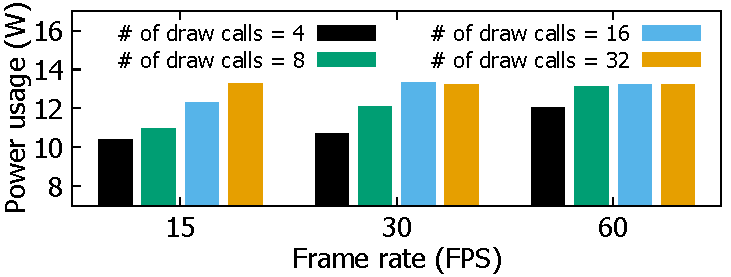
\includegraphics[width=0.8\linewidth]{frameRate_cropped}
    \vspace{-2ex}
    \caption{Power consumption for rendering the 69K-triangles Stanford Bunny
            with varying frame rates.}
    \label{fig:frame_rate}
\end{figure}

%%%%%%%%%%%%%%%%%%%%%%%%%%%%%%%%% 80 CHAR %%%%%%%%%%%%%%%%%%%%%%%%%%%%%%%%%%%%%%



\begin{figure*}[t]
    \vspace{-3ex}
    \begin{minipage}[b]{0.32\linewidth}
        \centering
        \subfigure[Total power]{
        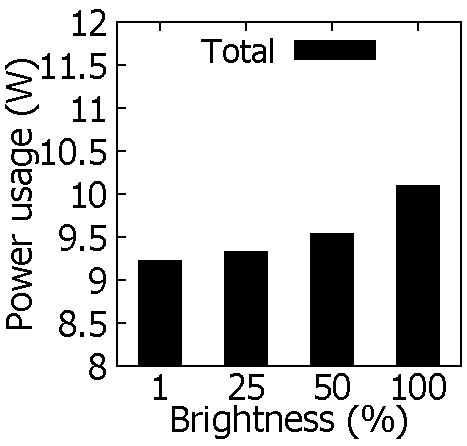
\includegraphics[width=0.45\linewidth]{brightness_total_cropped}
        \label{fig:brightness-total}
        }
        \hfill
        \subfigure[Headset power]{
        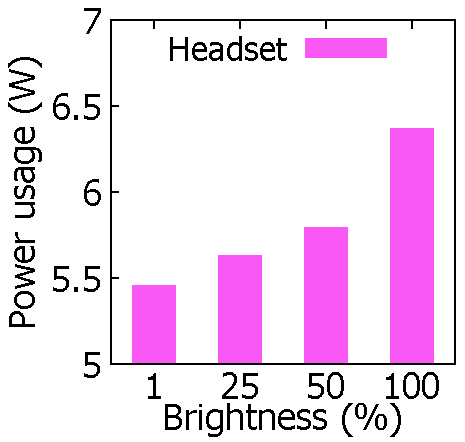
\includegraphics[width=0.45\linewidth]{brightness_headset_cropped}
        \label{fig:brightness-headset}
        }
        \vspace{-2ex}
        \caption{Impact of screen brightness on power consumption}
        \label{fig:brightness}
    \end{minipage}
    \hfill
    \begin{minipage}[b]{0.32\linewidth}
        \centering
        \subfigure[Total power]{
        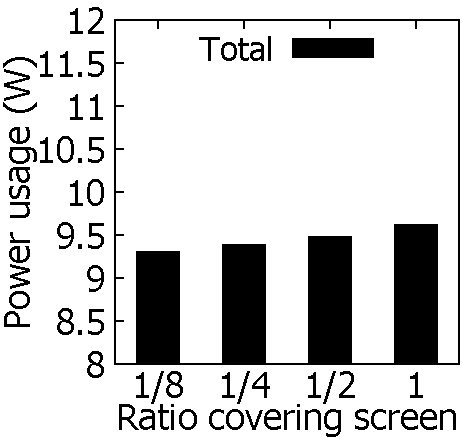
\includegraphics[width=0.45\linewidth]{objectSize_total_cropped}
        \label{fig:object_size-total}
        }
        \hfill
        \subfigure[GPU/memory power]{
        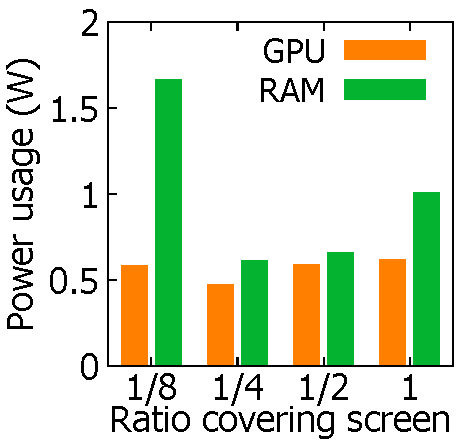
\includegraphics[width=0.45\linewidth]{objectSize_gpu_ram_cropped}
        \label{fig:object_size-gpu}
        }
        \vspace{-2ex}
        \caption{Impact of object size on power consumption}
        \label{fig:object_size}
    \end{minipage}
    \hfill    
    \begin{minipage}[b]{0.32\linewidth}
        \centering
        \subfigure[Total power]{
        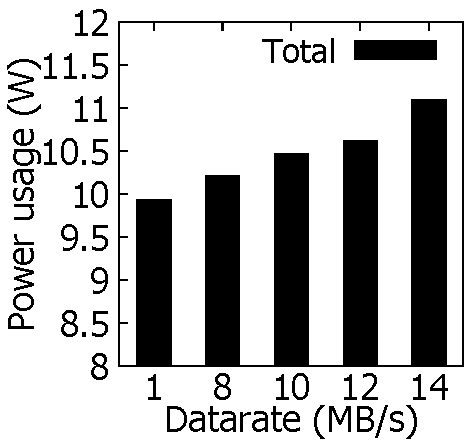
\includegraphics[width=0.45\linewidth]{datarate_total_cropped}
        \label{fig:datarate-total}
        }
        \hfill
        \subfigure[WiFi module power]{
        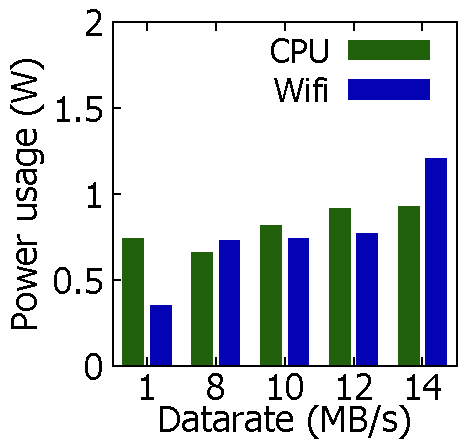
\includegraphics[width=0.45\linewidth]{datarate_wifi_cropped}
        \label{fig:datarate-wifi}
        }
        \vspace{-2ex}
        \caption{Impact of network data rate on power consumption}
        \label{fig:datarate}
    \end{minipage}
\end{figure*}

\spar{Screen complexity and frame rate}:
%
\figs\ref{fig:complexity} and \ref{fig:drawCall} together provide us hints
on how power usage can be effectively reduced on untethered AR headsets.
%
% A scene that requires many triangles will lead to high energy usage,
% regardless of whether the reason for screen complexity increase is due to
% a single complex object or many simple objects.
% %
% These results also provide an implication on how controlling the \emph{frame rate}
% of the object rendering process can impact the system's energy efficiency.
% %
% Given that high frame rates will issue more pipeline iterations and draw calls
% within a given time interval, the number of vertices to process is multiplied
% with the number of draw calls and the frame rate for a  time window, and 
% will heavily impact the system's energy consumption.
%
As shown previously, a scene that requires many triangles, either due to a single complex object or many simpler objects, will result in high power usage. This suggests that controlling the \emph{frame rate} can impact the system's power efficiency. In particular, high frame rates will require more pipeline iterations and draw calls within a given time interval, which will heavily impact the system's power consumption. This is shown in \fig\ref{fig:frame_rate} where we display 16K-triangle Stanford Bunnies using 15, 30, and 60 fps with 4, 8, 16, and 32 draw calls. We observed that as the overall complexity of the scene increases, the total power usage increases and saturates at $\sim$13~W.


%%%%%%%%%%%%%%%%%%%%%%%%%%%%%%%%%%%%%%%%%%%%%%%%%%%%%%%%%%%%%%%%%%%%%%%%%%%%%%%
%Note, however, that multiplying draw call count with per-object triangles 
%does not translate directly into energy usage.
%%
%If we compare the case with 13 draw calls of $\sim$3.7K triangles in
%\fig\ref{fig:drawCall} ($\sim$48.9K triangles in total) and the single draw call
%of the 48.6K triangle bunny in \fig\ref{fig:complexity}, the 13 draw 
%call case shows lower energy usage despite more triangles.
%%
%Thus, energy usage is \textit{not} a simple translation of the number of triangles.
%%
%Rather, it's a combination of per-object complexity, draw operation cost, and
%baseline energy usage, and their \emph{non-linear contribution} complicates 
%the energy optimization.
%%
%An example of such non-linearity lies in the memory alignment of modern processors.
%Specifically, processors will allocate memory in the power of 2 bytes for memory
%operations; thus, the memory usage for relatively complex objects (with a single
%draw call) can potentially be more burden to the processor compared to simple 
%objects with many draw calls, despite having the same number of total triangles.
%

%%%%%%%%%%%%%%%%%%%%%%%%%%%%%%%%% 80 CHAR %%%%%%%%%%%%%%%%%%%%%%%%%%%%%%%%%%%%%%

%\spar{What About Screen resolution?}:
%

%\raj{keep or toss to discussion? having a negative no-op result upfront seems odd. toss to discussion maybe. in a section called "other options?"}

%The screen resolution, has been shown previously to play a  critical role in varying the computational overhead~\cite{doi:10.1111/cgf.12956,Guenter:2012:FG}. However, similar to our inability to change the brightness levels programatically, the \mlo restricts all applications to a single 
%frame resolution (i.e., 1268x720).

%We plan to expand our studies with other resolution-controllable platforms to 
%observe the impact of screen resolution on energy usage as part of our 
%future work. 

%%%%%%%%%%%%%%%%%%%%%%%%%%%%%%%%% 80 CHAR %%%%%%%%%%%%%%%%%%%%%%%%%%%%%%%%%%%%%%

%%%%%%%%%%%%%%%%%%%%%%%%%%%%%%%%% 80 CHAR %%%%%%%%%%%%%%%%%%%%%%%%%%%%%%%%%%%%%%




\subsection{Display}

% \begin{figure}[t]
%     \centering
%     \includegraphics[width=0.8\linewidth]{brightness}
%     \vspace{-2ex}
%     \caption{Impact of screen brightness level on the HoloLens' energy 
%             consumption rate.}
%     \label{fig:brightness}
% \end{figure}

%Another 

A major power consuming component on mobile devices is considered to be the
display~\cite{187123,Anand:2011}. The {\mlo} uses LCoS displays, which could have very different power usage patterns from prior work studying LCD-based phone displays~\cite{Hwang:2017:RPO} and OLED-based displays~\cite{focusVR}.

An LCoS display is a micro-display that uses a ferroelectric liquid crystal 
layer, containing individual electrodes, on top of a silicon backplane. A CMOS chip controlling the electrode voltages is installed below the chip surface. A common base voltage for all the electrodes is supplied by a glass cover sitting on top. Such display technologies are also used in the Microsoft Hololens and the Google Glass~\cite{LiKamWa14GGlass}. 

%making this material suitable for AR displays 
%in the sense that the pixels that do not display objects remain transparent
%for users to freely observe the physical world.
%

To understand the power consumption of the display, we performed two experiments where we changed the
(1) \textit{display brightness} and (2) \textit{object size}. To study the impact of brightness, we configured the {\mlo} to show a pure white full screen image with different brightness. \fig\ref{fig:brightness} plots the power usage for brightness levels from 1-100\%. 

We observed that the headset's power consumption increases as the brightness increases. The 
difference in power usage between the lowest and highest brightness levels was $\sim$0.9~W (9\% increase). This suggests that dynamically adjusting
brightness can potentially improve the system lifetime~\cite{focus}.
%
However, currently, for the {\mlo}, the brightness setting can only be configured 
manually by the user and cannot be adjusted automatically by applications or on a per-object basis. Thus, while schemes to reduce brightness can improve the power consumption, we cannot use them in our specific implementation for {\mlo}.

%
%\jw{if we set the brightness level 0\%, hololens think it is empty screen,
%so it doesn't render it, so I set the brightness level 1\%, not 0\%.} 
%


% \begin{figure}[t]
%     \centering
%     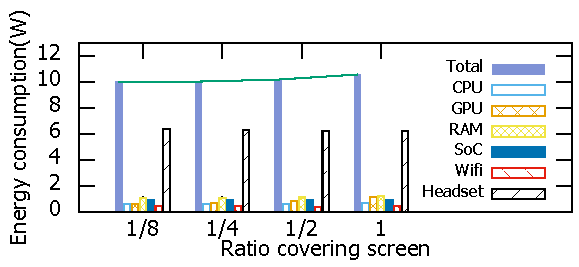
\includegraphics[width=0.8\linewidth]{objectSize}
%     \vspace{-2ex}
%     \caption{HoloLens energy consumption rate for different object 
%             sizes on the display.}
%     \label{fig:object_size}
% \end{figure}

Figure~\ref{fig:object_size} plots the power consumption when displaying 
different-sized solid squares on {\mlo} at maximum brightness level. We observed that as object size increases from 1/8 of the screen to 100\%, there was a $\sim$7\% increase in total power usage. Most of 
this was due to increased power consumption by the GPU and memory components, due to larger objects being rendered on the screen. We chose not to dynamically reduce the object sizes in our implementation, even though it could save power, as our studies revealed that users would quickly notice size differences between objects.

%\jk{Some more detailed discussions...}

%Despite drawing objects on a wider region, the object size itself did not play a 
%critical role in the energy consumption because there was no significant 
%difference in the \textit{geometrical complexity} of the object\footnote{We 
%confirmed that the impact of different colors (other than black - which 
%translates to a transparent image) on energy consumption were minimal.}.
%
%
%Note that with increasing object sizes, the LCoS display does activate larger
%areas, but, as we later show, this energy level of $\sim$490 mWh/10mins 
%represents the baseline energy usage of the HoloLens; thus, until the workload
%exceeds some threshold, the baseline energy is always used.


%However, we must take in consideration the fact that displaying a larger-sized
%image requires more pixel rendering at the HPU; thus, this energy usage pattern
%is actually a combination of both the display itself and the computational
%components. Furthermore, this is an application-driven factor, a piece of
%information that an intermediate layer cannot arbitrarily control.


%%%%%%%%%%%%%%%%%%%%%%%%%%%%%%%%% 80 CHAR %%%%%%%%%%%%%%%%%%%%%%%%%%%%%%%%%%%%%%


\subsection{Wireless Networking}

Finally, the wireless networking component is often considered to be a major power consumer in mobile systems with a number of solutions proposed to reduce its energy/power consumption~\cite{salsa,7034998,ALI2016173}. To investigate the impact of the networking module in mobile AR headsets, we connected the {\mlo} to a nearby WiFi AP and transmitted packets at data rates of 1MB/s, 8MB/s, 10MB/s, 12MB/s and 14 MB/s, respectively, over UDP, to a nearby sync server. Note that all other computational features were turned off, only with an empty white screen on the display. 

%During the experiment, we made sure that we achieve the target goodput to rule out the effect of TCP's rate control. 
%\raj{need to say why we stopped a such a low rate of 4MB/s. 780 Mbit/s 802.11ac should have ~100 MB/s rates. We are testing the energy consumption of a train by basically moving the wheels manually -- without firing up the engine -- and then saying that the energy increased slightly.... if TCP drops, just do a full line rate UDP blast and see what the energy looks like. no congestion or flow control. just 100\% networking usage.}

The results in \fig\ref{fig:datarate}, indicate that power consumption increases by $\sim$1~W as the data rate increases from 1MB/s to 14MB/s, and most of this increase is due to the CPU and WiFi modules. In this paper, we do not provide any schemes to optimize the power consumption of the wireless networking component for two main reasons; (1) there are already many proposed techniques~\cite{Qian2018, Qian2018TVP, Abari2017, Corbillon7996611} that we could reuse, and (2) more importantly, our survey of AR applications revealed that very few used the networking component in any significant way. Thus we focused our efforts on reducing the energy consumption of always-used components instead.

%\jk{Conclude this somehow...}



\subsection{Summary}
%
Our preliminary study using the {\mlo} suggests that a 3D object's 
geometric attributes, such as the object complexity and the frame complexity, 
along with the frame rate of the application, are crucial (and controllable) factors in modifying the energy usage of untethered AR headsets. In the next sections, we show how we design and evaluate a solution that uses these insights to effectively increase the battery lifetime of these devices.




%%%%%%%%%%%%%%%%%%%%%%%%%%%%%%%%% 80 CHAR %%%%%%%%%%%%%%%%%%%%%%%%%%%%%%%%%%%%%%
    
% \begin{comment}
%
% However, this is challenging for two major reasons. 
% %
% First, from an application developer's perspective, it is burdensome to take 
% such optimization factors in consideration while designing an application
% for every application they design. Developers would rather spend time on
% the attractiveness of the visual content than on energy efficiency.
% %
% This suggests for a dedicated and transparent (and optionally enabled)
% computational layer beneath the application layer (and above the graphics stack)
% for optimizing the object rendering process to achieve maximal energy efficiency
% without putting the responsibility on the application developer.
% %
% Second, even if such a layer was available, %on a technical perspective, 
% there are additional technical challenges:
%
% \begin{itemize}[leftmargin=*]
%     \item {\bf Knowing exactly what will be drawn on the frame.}
%         Optimizing the system for energy efficiency using 3D object geometric
%         attributes would require this, but this information is difficult to 
%         capture in a closed system 
%         while requesting minimal modifications to the application.
%
%     \item {\bf Preserving the user experience.} 
%         While achieving energy efficiency is attractive, making sure that
%         the user enjoys perceptually high quality objects is still the most
%         important requirement. Therefore, system optimization for energy efficiency
%         should only occur to a level where the user perception on the 
%         application experience is minimally affected.
%
%     \item {\bf Light-weight and computationally tractable.}
%         Applying a precise, but heavy algorithm to compute the optimal
%         vertex-quality relationship's tradeoff may not be desirable since
%         heavy computation itself can be a burden on the energy usage.
%         Therefore, light-weight mechanisms are required.
%         For example, using embedded sensing information to limit the rendering
%         scope can be an effective way to limit the computational costs. 
%   
% \end{itemize}
%
% \end{comment}

%%%%%%%%%%%%%%%%%%%%%%%%%%%%%%%%% 80 CHAR %%%%%%%%%%%%%%%%%%%%%%%%%%%%%%%%%%%%%%


\section{Low-power Graphics Library}
\label{sec:system}

    
%%%%%%%%%%%%%%%%%%%%%%%%%%%%%%%%% 80 CHAR %%%%%%%%%%%%%%%%%%%%%%%%%%%%%%%%%%%%%%

The results from our preliminary empirical studies suggest that a combination of
various geometric attributes (e.g. number of triangles and draw calls) and 
system-level parameters (e.g., frame rate) need to be considered when optimizing 
the AR application's graphics rendering requests for power efficiency.
%
Moreover, if there are several 3D objects to be displayed, each object may 
need to be optimized separately depending on their texture or motion 
characteristics. Managing this individually for each
application may be a significant burden and learning curve for the 
developers.
%
Therefore, having a dedicated library implementation that manages object
rendering, while considering various power-affecting factors, can be
beneficial for mobile AR application development.
%
Such operations should be kept transparent to the application, the added 
computation should be minimal, and should take in consideration the user perceived object quality.
%
To this end, we summarize the design goals of a low-power graphics library for 
mobile AR headsets as follows:


\begin{itemize}[leftmargin=*]

    \item Maintain a transparent pass-through layer between the native graphics
        library and the application for various programs to easily inter-connect
        without putting the responsibility on the application developer.
    
    \item Light-weight and computationally tractable schemes are needed
        to assure that power and resource usage of the 
        implementation does not outweigh its power savings.
    
    \item Manage 3D object display based on how the user perceives
        (both the physical visibility and quality) the AR environment.
        While achieving poewr-efficiency is attractive, maintaining application quality is still important.
    
%    \item Offer a controllable threshold for 3D object quality to satisfy 
%        diverse user/application requirements.
\end{itemize}


\begin{figure}[t]
    \centering
    \vspace{-1ex}
    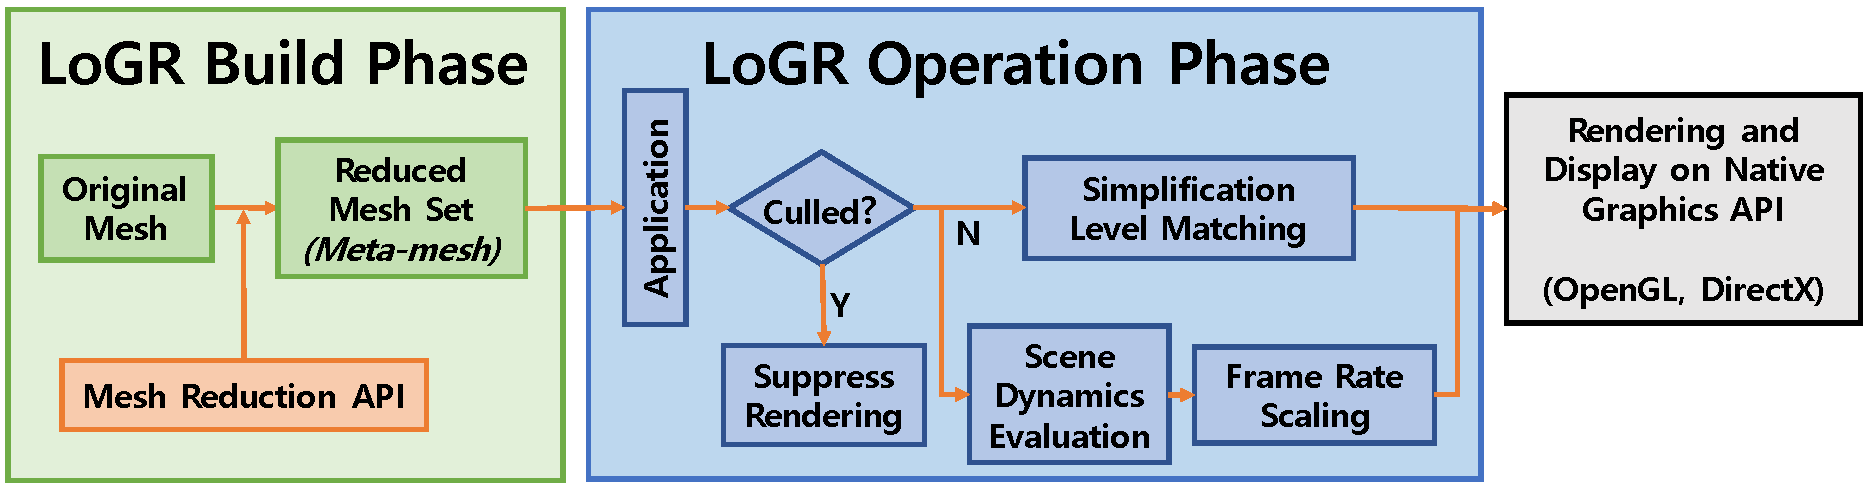
\includegraphics[width=1\linewidth]{scheme_cropped}
    \vspace{-2ex}
    \caption{{\myit} -- 
           the architecture and its functions.}
    \label{fig:lpglDiagram}
\end{figure}

With these goals in mind, we design {\myit}, a Low-power Graphics Library
for mobile AR headset applications.
%
In the software stack, {\myit} is positioned between the application and the 
system's native graphics library (e.g., OpenGL, DirectX)
(\fig\ref{fig:lpglDiagram}).
%
To the application, {\myit} provides OpenGL ES compatible front-end APIs.
%
For an application that uses these APIs, {\myit} intercepts the 
graphics-related calls to understand what the application targets to draw
(e.g., type/location of drawing, quantity of models).
%
In addition, {\myit} obtains user view points from the headset to gather
user perception physics (e.g. angle of sight, gaze).
%
Then, these information are combined to optimize the drawing process with respect 
to other system parameters, such as the frame rate and geometric complexity, so
that power usage is reduced while minimizing user perceived quality loss.
%
The following subsections provide details on the {\myit} design.


%%%%%%%%%%%%%%%%%%%%%%%%%%%%%%%%% 80 CHAR %%%%%%%%%%%%%%%%%%%%%%%%%%%%%%%%%%%%%%

\subsection{{\myit} Front-end APIs}

Front-end APIs of {\myit} are designed to be compatible with the OpenGL
ES 3.0 APIs~\cite{opengl}. 
%, while adding a few additional {\myit}-specific APIs.
%
This results in no changes to the application's code and allows {\myit} 
to easily intercept and capture the contents to be drawn on the display.
%
Through the APIs, {\myit} hooks to the graphics-related calls from the application
and passes appropriate information to its sub-modules for further processing, prior to sending commands to the system's native graphic library.
%
%Specifically, the current implementation of {\myit} offers calls for the
%graphics library's geometry-related functions.


%%%%%%%%%%%%%%%%%%%%%%%%%%%%% REWRoTE %%%%%%%%%%%%%%%%%%%%%%%%%%%

%A major design goal of {\myit} is to achieve complete application transparency, meaning that we target to enforce no changes to the application code itself to use the {\myit} capabilities. 

To achieve this transparency, we design our software so that all {\myit} functionalities are enabled through compiler configurations. The application developer simply makes changes to the compiler configurations to use {\myit}, and at compile time, the source code binary and necessary 3D objects are modified to support the added features of {\myit}. 
%
These, compile time configurations allow {\myit} to intercept all graphics-related calls prior to entering the native graphics stack. Specifically, through this process we (1) initialize {\myit}, (2) configure a command queue in which application API calls can be gathered before being pushed to the system graphics stack, and (3) load a mesh with different complexities to perform mesh simplification as we will detail in Section~\ref{sec:mesh}. 


%\fig\ref{fig:api} presents {\myit}-specific APIs and an example
%OpenGL compatible wrapper API ({\small\tt glVertexAttribPointer()}) supported by 
%{\myit}.
%
%Here, {\myit}-specific APIs are special purpose APIs used for operating {\myit}.
%{\small\tt lpglInit()} initializes internal data structures such as the command 
%queue for hooking to a graphics call. {\small\tt lpglInit()} must be called to 
%use the {\myit} functionalities. 
%
%The command queue, a core data structure, gathers the application's API calls 
%until the {\small\tt lpglCommit()} command is issued. {\small\tt lpglCommit()}
%then pushes the commands through the {\myit} procedures and passes the (modified)
%commands to the native graphics stack.
%
%While OpenGL compatible APIs mimic native graphics API calls, in reality, calls
%made from the application are put into the {\myit} command queue for modifications
%at {\myit} components once {\small\tt lpglCommit()} is issued.
%
%In addition, when objects are created at the application, loading commands are 
%called to place the objects' geometries to the graphics buffer for the draw calls 
%to execute. At this phase, we introduce a third {\myit} command, {\small\tt 
%lpglLoad()}. This call allows {\myit} to simplify a target object's complexity as 
%we will detail in Section~\ref{sec:mesh}. 
%%%%%%%%%%%%%%%%%%%%%%%%%%%%%%%%%%%%%%%%%%%%%%%%%%%%%%%%%%%%%%%%%


%\begin{figure}[t]
%    \centering
%    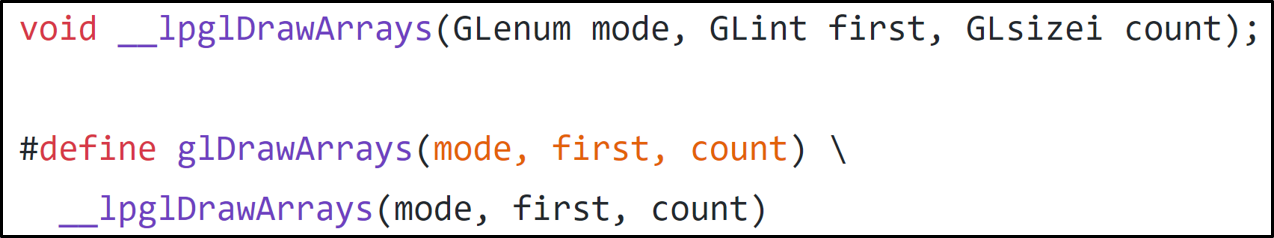
\includegraphics[width=1\linewidth]{lpglSourceCode}
%    \vspace{-2ex}
%    \caption{A Sample API example provided by {\myit}.
%            }
%    \label{fig:api}
%\end{figure}


% Internally, the native calls are preprocessed.
% In detail, we defined preprocessor function to mimic native OpenGL APIs.
% If application developer types OpenGL API for example 
% {\small\tt glDrawElementsInstanced()}, it is resolved to source code which 
% calls {\small\tt \_\_lpglDrawElementsInstanced()} by preprocessor.
% {\small\tt \_\_lpglDrawElementsInstanced()} function pushes their given 
% parameters to command queue.


OpenGL-compatible front-end APIs supported in {\myit} consists of two parts: 
APIs for initializing the drawing data, and APIs for the actual drawing.
%
The calls to the former contain information on what objects will be drawn,
%
including vertices and topology information. 
%(c.f., \fig\ref{fig:lpglDiagram}).
%
APIs for the actual object drawing are again divided into two categories:
%
transformation APIs apply geometric transformation
(e.g., scaling, rotation, translation) to the target object, and
%
draw calls send commands to draw objects to the GPU.
%by applying the transform functions to the vertex buffer configured in the
%initialization phase.


%%%%%%%%%%%%%%%%%%%%%%%%%%%%%%%%% 80 CHAR %%%%%%%%%%%%%%%%%%%%%%%%%%%%%%%%%%%%%%


\subsection{Mesh Simplification}
\label{sec:mesh}

As we saw in the preliminary studies, the number of triangles that consist 
a 3D object (i.e., object complexity) heavily impacts the power usage of a mobile AR application. 
%
However, when displaying multiple complex objects in a single scene, often the 
user's perception (e.g., direction of sight or gaze) is towards only a subset 
of the objects.
%
Therefore, it makes sense to simplify objects that are out of the user's 
focal angle to minimize the power used for processing these objects.

To do so, we start by identifying the number of triangles that an application 
intends to draw using the {\small\tt glBufferData()}
and {\small\tt glVertexAttribPointer()} calls in the OpenGL APIs,
which provides vertices and topology information. 


Next, to reduce the number of triangles that consist an object while 
maintaining visible quality, we apply \emph{mesh simplification}.
%
Mesh simplification %a well-studied topic in the graphics research community, 
is used in various graphics applications to minimize computation costs for less-focused
objects. Among various methods, we used Audodesk Maya's Mesh Reduction
API~\cite{polyReduce}. %The use of other methods are also easily applicable.


%%%%%%%%%%%%%%%%%%%%%%%%%%%%% REWRoTE %%%%%%%%%%%%%%%%%%%%%%%%%%%

However, mesh simplification can be computationally heavy when performed on
the mobile headset itself. Therefore, all potentially displayed objects in {\myit} are
simplified \textit{in compile time} to create two 
additional versions of simplified meshes. Here, one version is a ``less'' 
simplified version (level 1 simplification) and the other is heavily simplified 
(level 2). For simple memory loading, the geometries of the original, 
level 1 and level 2 simplification meshes are combined to form a ``meta-mesh'' of an object.
%All 3D objects will have two aliases of the original mesh, a level 1 mesh and a level 2 mesh.
We note that some applications dynamically load 3D objects in run-time. To reduce 
object complexity for those not simplified in compile time, {\myit} also includes
a light-weight mesh simplification scheme based on Quadric Error Metrics~\cite{Garland98}
to reduce mesh complexities in run-time.

In operation, the meta-mesh of the target object is loaded to the memory upon 
a display request. As soon as a decision is made on what version of the
object should be displayed, the meta-mesh is split, and only the geometry for the
target complexity mesh is passed to the GPU.% memory for further processing. 

%%%%%%%%%%%%%%%%%%%%%%%%%%%%%%%%%%%%%%%%%%%%%%%%%%%%%%%%%%%%%%%%%%%%

In determining when and what version of the object will be displayed, we utilize 
gaze tracking or head orientation information provided by the mobile headset. 
Based on geometric information on how far an object is away from the user's focal 
point, we divide the user's field of view (FOV) in three: core focal 
angle, near peripheral sight, and far peripheral sight. 
%
Assuming that the user's core focal angle is within $\epsilon^\circ$ from the
current focal point extracted from the gaze tracker or head orientation 
information, objects beyond this angle distance can be simplified. If the object 
is located 1-3$\times\epsilon^\circ$ away from the focal point, we present
the level 1 simplified mesh, and use level 2 for all objects farther away. 
%
%Based on findings from previous literature~\cite{Strasburger11}, we set $\epsilon^\circ$ to $10^\circ$ and validate this using experiments in Section~\ref{sec:inlab}.



%%%%%%%%%%%%%%%%%%%%%%%%%%%%%%%%% 80 CHAR %%%%%%%%%%%%%%%%%%%%%%%%%%%%%%%%%%%%%%

\subsection{Frame Rate Control}

Our preliminary results show that frame rate has significant impact on the 
system's power usage. However, its control should be done with care since 
low frame rates may drastically drop the user perceived quality.
%
%Thus, {\myit} aims to guarantee that users' application experience is only
%minimally (if at all) affected.
%
Frame rate control in {\myit} is designed based on the intuition that frame rate 
need not be constant across all visual contents~\cite{Lim18Adaptive}.
%
It should be kept high to maintain the original quality for contents that change
frequently (e.g., high level of scene dynamics), but can be lowered without loss
of user-perceived quality when contents are less dynamic.
%
To exploit this idea, {\myit} implements a {\it Scene Dynamics Scoring Module},
which determines and quantifies the scene dynamics of frame contents using the 
scene's geometric information.
%
Based on this score, the {\it Reactive Display Complexity Control Engine} 
(Section~\ref{sec:rdcc}) can determine an appropriate frame rate.
%for the display content.

For example, if we define a scene's dynamics as the difference 
between subsequent frames, image-based schemes that use 
full contextual information, such as the structural similarity (SSIM) or peak signal-to-noise ratio (PSNR) can be used~\cite{ssim,psnr}.
%
However, they require significant amount of computation,
% to calculate features from the entire screen, and 
thus unsuitable for resource limited mobile devices~\cite{ssim,Hwang:2017:RPO}.
%due to the computational and latency overheads.
%
% Work by Hwang et al. also realize such complexity issues and use grayscale 
% images to reduce the computation cost~\cite{\cite{Hwang:2017:RPO:3117811.3117841}}. 
%
% To compute frame similarity in real-time despite the complexity,
% image-based schemes may use lower-resolution images rather than full resolution, 
% but this would still make it difficult to adaptively control the granularity.
%
% Applications that show detailed level changes would require {\myit} to monitor
% changes in the image in finer granularity compared to rough image-changing 
% applications. For the applications that are less sensitive, performing 
% fine-grained computation can be a waste of resources.
%
Furthermore, with these schemes, it is difficult to compute scene dynamics until the frame is fully rendered for object rendering applications, .
%and the image is available in the display buffer. 
We find this and the memory copy from the GPU's frame buffer as computational waste.

Moreover, image-based metrics may not be sensitive enough for small portions
of changes in the scene. Take a case in which a small object such as a bullet
passes through the user's scene. The bullet will travel fast, but if we compute 
the SSIM/PSNR for the entire frame, the contextual changes will only be marginal. 
Such schemes can suggest that there is
only a small level of dynamics and decrease the frame rate accordingly. In 
applications where drawing is done on an object-basis, we need a scheme 
more centered towards the objects themselves, rather than the entire frame image. 

%are not sensitive to the small portion of changes of whole scene.
%In an example of a scene which a man is shooting gun,
%even if the bullet would be fast enough but it would be evaluated as a little changes and set lower framerate. However from user's point of view, the bullet will be blown with stuck, which can be expected to have a negative impact on the user experience.


Such observations led us to propose and design a \emph{Distance-based frame 
dynamics scoring module}, an \emph{object geometry-based} light-weight approach 
for determining scene dynamics.
%
In our approach, the scene dynamics is defined as the maximum distance change of 
objects within two consecutive frames computed over all objects in the scene. Note
that this distance is defined 
%in the 2D coordinate space 
on the user's view point perspective.
%, not in the global 3D space. 
Therefore, even when the object is stationary and the user's view point changes 
(e.g., motions with the mobile AR device), the the dynamics can be captured.
%
To minimize computation costs, instead of using the original detailed coordinates 
of the 3D object, we set a ``bounding-box'', which is a box that best fits all the 
coordinates of the original object, and only compute the distance based on the 
box's center point. 
%
Such an approach allows {\myit} to compute the dynamics level of the scene 
before the scene is rendered, to suppress any unnecessary rendering and memory 
copy operations.

% However geometry-based method can not detect color and texture differences for non-moving objects. \jw{How about move the story about color and texture to discuss section?}
%

% \jk{add geometry distance-based method...}

% \jk{note the fact that this approach can capture things that PSNR/SSIM cannot capture. We are not focusing on the entire frame but if one object makes a fast motion, even if the object is small, we see the need to increase the frame rate.}

% \jk{limitation of geometry-based schemes is that we cannot capture changes in color/texture for non-moving objects}

%%%%%%%%%%%%%%%%%%%%%%%%%%%%%%%%% 80 CHAR %%%%%%%%%%%%%%%%%%%%%%%%%%%%%%%%%%%%%%

\subsection{Culling}

In addition to frame rate, the number of draw calls also impact the power 
consumption of a mobile AR headset.
%
Issuing draw calls are essential for drawing objects to the display, but 
executing draw calls for objects that cannot be physically seen 
(e.g., object out of current scene boundaries) would be a waste.
%
The most widely used graphics pipelines already exploit ``view frustum culling'' 
to account for such cases~\cite{}. The process of culling determines whether or not there 
is a chance for the target object to be observed 
%in the current scene, 
and suppresses the drawing if not.
%
%Specifically, in view frustum culling, once triangles complete vertex shading,
%the culling module checks if the object is outside of the ``view frustum'' 
%constructed using the gaze direction, FOV, and visible range.
%
%If an object is inside the view frustum, it is visible. Otherwise,
%culling suppresses the remaining graphics pipeline tasks, allowing the 
%system to conserve resources. 


%While culling itself is very important in saving energy and is already widely
While culling itself is already widely used, we've identified a point in which 
the main philosophy of ``not processing unseen objects'' can be further exploited 
to reduce power consumption even more.
%
In currently used view frustum culling, when a user is observing an object in the $x^\circ$ field, objects in the $x+180^\circ$ range 
will still be processed and pay the computation cost up to the point where the object geometries are known to the graphics library after being fully transformed to the 3D space.
%
%vertex shader
%before it is discarded. \jk{change this part a bit...}
%
%Surprisingly, this occurs for all well-known graphics libraries 
%since the geometry of the object is not known to the library until the 
%object is transformed on the 3D space.
%
However, objects beyond peripheral vision can not be seen, and we propose to 
eliminate \textit{all} the waste in the culling process.


Again, we exploit the user perception data, geometry information 
of all objects, and apply the bounding box-based approach.
%
By doing so, instead of transforming all vertices to the 3D space, we can selectively transform just the eight corner points that consist the bounding box. 
%
We infer the user's position in the 360$^\circ$ space, and use it to 
compute the angular distance $\tau^\circ$ between the user's view point direction 
vector and the vector of the object bounding box's center position.
%
Then, given a typical user's maximum FOV, if $\tau^\circ$ is not included in the 
FOV, we determine that there is no chance for the target object to be seen in the 
current scene.
%
Using this simple method, {\myit} improves view frustum culling and suppresses the
entire graphics pipeline process.

%\jk{I don't see how this is different from baseline}

%%%%%%%%%%%%%%%%%%%%%%%%%%%%%%%%% 80 CHAR %%%%%%%%%%%%%%%%%%%%%%%%%%%%%%%%%%%%%%

\subsection{Reactive Display Complexity Control}
\label{sec:rdcc}

%\jk{Change so that different levels are reflected in the text.}

%So far, we have discussed how {\myit} captures information from the application,
%how the meshes can be simplified and displayed based on the user's sight,
%how we quantify frame dynamics to control the frame rate,
%and how the culling process can be optimized to minimize the number of draw calls.
%
The mesh simplification, scene dynamics scoring, and culling techniques
discussed until now are designed based on the idea that we can utilize the
relationship between the user's view point (from the gaze tracker) and the 
object's geometry.
%
To effectively combine all {\myit} features, 
we design the Reactive Display Complexity Control (RDCC) engine.
%
The RDCC engine offers a framework that exploits the three core features of
{\myit} with minimal computational overhead, and provides a fine-grained 
display control environment. 
%
Through RDCC, {\myit} reactively controls graphics-related parameters 
based on the user's perception of the scene. 

A key idea of the RDCC engine in {\myit} is to focus the computation on only the 
bounding-box surrounding the geometry rather than the full geometric information.
%
Take the culling process for example, which is interested in identifying 
whether the target object is within the user perceived scene or not.
%
Given that the bounding box provides the minimum and maximum points of the object,
if we simply identify that the bounding box is outside the user's sight, we can
easily remove this object from the graphics pipeline.
%
Similarly for frame rate control and mesh simplification, the RDCC engine makes
its decisions based on features (e.g., scene dynamics or object position) extracted from the bounding box. 

Overall, RDCC operates as follows. For each object draw call, the culling process first takes place after identifying the object's bounding box. Then a mesh of 
a proper detail (e.g., original object or simplified mesh) is presented 
after determining that the object is currently within the core focal angle or near 
peripheral angle. Finally, the target frame rate is set 
based on the objects' dynamics in the scene to project them through native graphics 
library's drawing APIs.


%As for the frame rate, the RDCC engine determines when the next frame will be 
%displayed based on the current value of the frame dynamics score. 
%
%High level of dynamics will result in high frame rate, and a low dynamics score
%will lead to a lower frame rate.
%
%This decision is based on a set of parameters which determine at what 
%dynamics level the frame rate will ``shift" to a different level.


%Finally for mesh simplification, the RDCC engine takes the role of confirming
%if an object's bounding box is within $\epsilon^\circ$ of the center of focus 
%or not with respect to the head direction
%extracted from the gyroscope sensor.
%
%Since, the bounding box of an object is a common feature that all three 
%components in {\myit} use, the RDCC engine extracts this 
%information prior to processing the object in different components. 


%%%%%%%%%%%%%%%%%%%%%%%%%%%%%%%%% 80 CHAR %%%%%%%%%%%%%%%%%%%%%%%%%%%%%%%%%%%%%%

%\subsection{{\myit} Parameter Selection}
%\label{sec:parameters}


%Given the design discussed until now, 
%it is important that {\myit} offers proper controllable parameters so that 
%its functionalities can be effectively exposed.
%
%Current implementation of {\myit} offers three major parameters.
%
%First is $d_B$, the binary tree depth parameter for controlling the mesh 
%simplification level.
%With a small $d_B$, the 3D objects are represented with only a small number of
%voxels, which reduces the quality of the object, but maximizes energy efficiency.
%A large $d_B$ on the other hand, will provide a fine-grained and detailed 
%object projection, but limits the energy reduction.
%
%In this phase, $min_{vx}$ can also be configured to set the level of filtering
%adjacently created triangles. While this value can be variable, current 
%implementation of {\myit} fixes this value to 30 based on a number of object
%quality measurements.


%The second controllable parameter in {\myit} is $d_Q$, the depth metric for
%determining frame dynamics. A high $d_Q$ will provide a very detailed 
%summary of the changes occurring on two consecutive frames, while a small 
%$d_Q$ will provide information on easily noticeable, larger differences.
%
%The resulting frame dynamics score $DS_n$, is compared with a threshold $DT_n$
%that specifies when the RDCC engine should determine to transition to a 
%new display frame rate.
%
%This process should define a set of thresholds for shifting the frame rate
%from $FR_1$ to $FR_2$, for example.
%When configuring the target frame rate $FR_n$ in multiple steps, thresholds 
%$DT_n (n=1,2,3,...)$ should be defined for each frame rate transition state. 


%Note that the currently {\myit} allows the application to 
%choose these parameters, and does not offer preset values.
%Configuring preset values or autonomously adapting these parameters on a 
%per-user (or-per application) basis requires deeper user studies and we 
%leave this as part of future work. 

%%%%%%%%%%%%%%%%%%%%%%%%%%%%%%%%% 80 CHAR %%%%%%%%%%%%%%%%%%%%%%%%%%%%%%%%%%%%%%


\section{In-lab Experiments}
\label{sec:inlab}

%%%%%%%%%%%%%%%%%%%%%%%%%%%%%%%%%%%%%%%%%%%%%%%%%%%%%%%%%%%%%%%%%%%%%%%%%%%%%%%%

We start our evaluations of {\myit} using controlled in-lab experiments to  analyze and understand the performance of {\myit} under  different experimental settings. Specifically, we measure the power usage for different culling angles, 
focal angles, and motion dynamics to capture the impact of each {\myit} feature,
(1) culling, (2) mesh simplification, and (3) screen dynamics-based frame rate 
control, respectively. We also gathered qualitative measurements using a small-scale user study of five participants to understand how parameter changes in the three  criteria affects the perceived object quality to determine the appropriate values for our application-oriented user studies (discussed in Section~\ref{sec:userstudies}). 


%%%%%%%%%%%%%%%%%%%%%%%%%%%%%%%%%%%%%%%%%%%%%%%%%%%%%%%%%%%%%%%%%%%%%%%%%%%%%%%%

\subsection{Culling Angle}

\begin{figure}[t]
    \centering
    \vspace{-1ex}
    \subfigure[Total power usage]{
       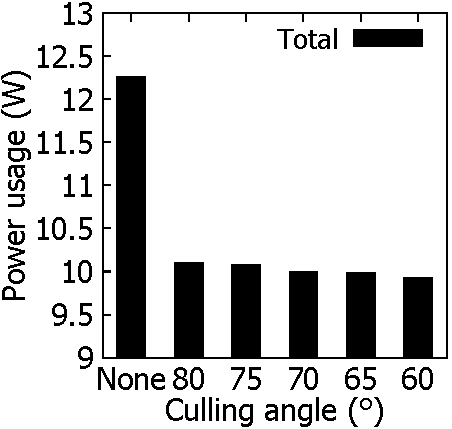
\includegraphics[width=0.45\linewidth]{Culling_cropped}
        \label{fig:lpgl-cullingangle}
    }
    \subfigure[GPU/memory power usage]{
        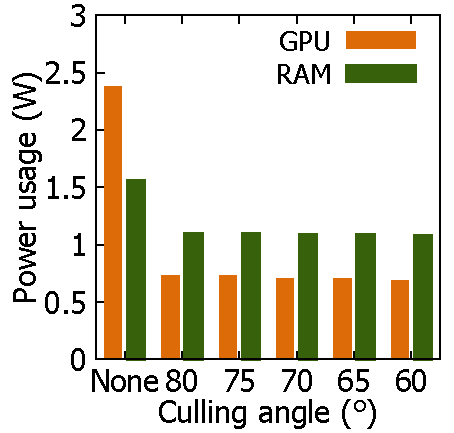
\includegraphics[width=0.45\linewidth]{Culling_GPU_RAM_cropped}
        \label{fig:lpgl-cullingangle-gpu}
    }
    \vspace{-2ex}
    \caption{Power consumption for enabling
            {\myit}'s culling at different angles.}
    \label{fig:lpgl-cullingangle-all}
\end{figure}


To identify the optimal culling angle for the {\mlo}, we first built an application to display 72 small bunnies horizontally with the center bunny (right in front of the user's field of view) colored in green and the other 71 colored in white, arranged evenly in a 360$^\circ$ circle around the participant -- with each bunny separated by its neighbor by $360/72=5^\circ$. During the experiment, we asked each participant to focus their attention on the green bunny and inform us when they noticed something changing in the scene. We then slowly removed bunnies from the scene starting with the leftmost and rightmost bunnies (they were always removed in matching pairs) until the participant noticed something changing in their visible scene.

This experiment was designed to identify the visual angle at which participants could notice changes to the scene with their peripheral vision. This angle is important to know as objects outside this noticeable area can be culled by {\myit} (i.e. not rendered) to save power. On the {\mlo}, the effective maximum field of view is 80$^\circ$ -- thus we started our tests from 80$^\circ$, as anything larger would not be visible anyway (as the {\mlo} would not display it).

Figure~\ref{fig:lpgl-cullingangle-all} shows the reduction in power consumption as the culling angle moves from ``None'' to 80$^\circ$ and lower. We observe that, depending on the scene complexity, significant amounts of power (20\% or more) can be saved by not rendering objects that cannot be seen by the user. However, this culling has to be balanced with usability. From our study, we noticed that, due to the small field of view of the {\mlo}, any culling in the visible area was immediately noticed by the participants. Thus, despite increased power savings potential, to maintain the user experience, we set the culling angle for the {\mlo} to 80$^\circ$ (to match its small field of view) in all future experiments.


%We designed a static application is spreading many white little bunnies in front side and middle green bunnies to focus the middle side. Under such conditions, we target to observe the performance of {\myit}'s culling algorithm as it analyzes the angle of the current scene. Specifically, we use tiny bunnies. When changing culling angles, we want to check fine angles for finding a suitable parameter. The focus angle's level 1 is 10$^\circ$ and level 2 is 60$^\circ$ is based on our preliminary quality studies. From the bars in \fig\ref{fig:lpgl-cullingangle} we can see that even at 80$^\circ$ (performance-wise worst case for {\myit}), when applying {\myit}, the energy consumption is lower compared to the baseline. 


%%%%%%%%%%%%%%%%%%%%%%%%%%%%%%%%%%%%%%%%%%%%%%%%%%%%%%%%%%%%%%%%%%%%%%%%%%%%%%%%

\subsection{Focal Angle}


\begin{figure}[t]
    \centering
    \vspace{-1ex}
    \subfigure[Total power usage and 5-point Likert-scale score on scene quality]{
       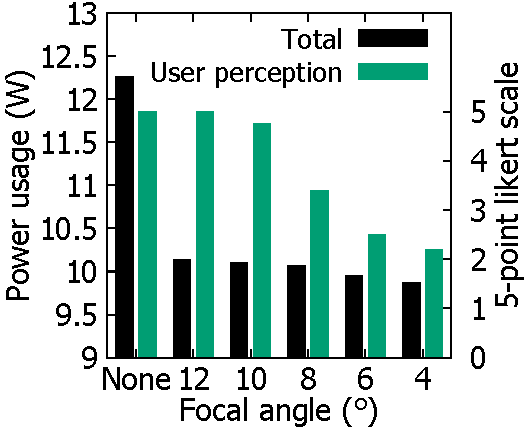
\includegraphics[width=0.49\linewidth]{Focus_cropped}
        \label{fig:lpgl-focusangle}
    }
    \subfigure[GPU/memory usage]{
        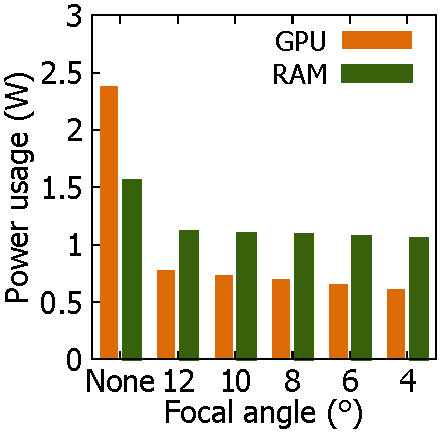
\includegraphics[width=0.409\linewidth]{Focus_GPU_RAM_cropped}
        \label{fig:lpgl-focusangle-gpu}
    }
    \vspace{-2ex}
    \caption{Power consumption and scene quality perception scores for
            varying core focal angles.}
    \label{fig:lpgl-focusangle-all}
\end{figure}

{\myit} defines two types of focal angles: \textit{peripheral focal angle} and \textit{core focal angle}. For objects that are farther away
than the peripheral focal angle, a very simple mesh is presented 
(level 2 simplification), and for objects within the \textit{core focal angle} 
the highest quality mesh is presented. If the object is located between these two angles, a level 1 simplified mesh is displayed. We set the peripheral focal angle to 60$^\circ$ based on findings from previous literature~\cite{Grosvenor07, Bhise11}, and used the culling angle application to understand the impact of changing the core focal angle on the power and user perception, except for this experiment, we placed the bunnies $2^\circ$ apart to observe any effects at  finer granularity.


During the study, we randomly set the core focal angle to different values and asked the participants to focus on the green bunny in the center and rank the quality of the scene using a 5-point Likert scale (very low: 1, very good: 5). With decreasing core focal angles, the bunnies that are located close to the user-focused green bunny will start to be presented as a simplified mesh. Our results, shown in \fig\ref{fig:lpgl-focusangle-all} for both power consumption and user perceived quality, suggest that the participants started to quickly notice changes when the core focal angle was smaller than 10$^\circ$. Again, similar to the culling angle, despite the power benefits of a narrow core focal angle, we set the focal angle to 10$^\circ$ to minimize the usability impact.


%
%However, based on the findings from the previous experiment, we fixed the 
%culling angle at 80$^\circ$.
%(the angle distance from the user's focal point up to where the high quality objects are drawn) 
%

%
%


%From our user study, we noticed that having a core focal angle higher than
%10$^\circ$ did not show any differences on the user perception levels.
%In \fig\ref{fig:lpgl-focusangle} we present the energy consumption for the 
%{\mlo} for different core focal angle values. If an object resides within the
%core focal angle, a high quality representation of the 3D object is presented 
%on the screen. Therefore, as we decrease the angle, we see lower energy usage 
%at a device-scale, mostly due to the reduction of energy usage at the GPU and
%memory. Nevertheless, given that the goal of {\myit} is to maintain the user 
%perception while reducing energy consumption, we keep the core focal range to
%10$^\circ$ in the following experiments.


%We start changing level 1 focal angle at 12 based on our preliminary studies. Because people don't noticed that something is strange when focal angle is over 12. We can see that \fig\ref{fig:lpgl-focusangle}, increasing level 1 focal angle, energy usage is increased.


%%%%%%%%%%%%%%%%%%%%%%%%%%%%%%%%%%%%%%%%%%%%%%%%%%%%%%%%%%%%%%%%%%%%%%%%%%%%%%%%

\subsection{Object Speed and Frame Rate}


\begin{figure}[t]
    \centering
    \vspace{-1ex}
    \subfigure[Total power usage and achieved frame rate for varying object speeds]{
       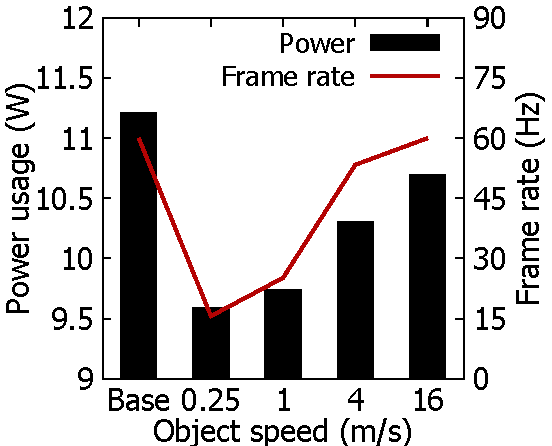
\includegraphics[width=0.49\linewidth]{objectSpeed_cropped}
        \label{fig:lpgl-objSpeed}
    }
    \subfigure[GPU/memory usage]{
        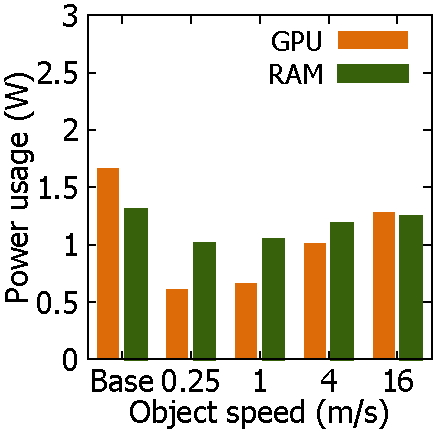
\includegraphics[width=0.409\linewidth]{objectSpeed_GPU_RAM_cropped}
        \label{fig:lpgl-objSpeed-gpu}
    }
    \vspace{-2ex}
    \caption{Power consumption and scene quality perception score for varying object speeds.}
    % which impact {\myit}'s frame rate control.}
    \label{fig:lpgl-objSpeed-all}
\end{figure}


Next, to investigate the impact of {\myit}'s dynamic frame rate control, we conducted an experiment where four 69K triangle bunnies are moved up and down the scene.  We varied the speed of the bunnies from 0.25-16~m/s keeping each bunny 5 meters away from the user. At 0.25~m/s (low dynamics), we expect {\myit} to use a low frame rate (15 fps), while at 16~m/s, we expect {\myit} 
to use the maximum frame rate (60 fps). {\myit} uses three levels of frame rates, 15, 30 and 60 fps, and we configured it, based on our initial user tests, to move from 15 to 30 fps if, across two frames, at least one object moves across more than 15\% of the entire scene. If an object moves across more than 30\% over two subsequent frames, we set the frame rate to 60 fps.
%
From the results, shown in \fig\ref{fig:lpgl-objSpeed-all}, we note that even at 60 fps displaying the same objects, {\myit}'s power consumption is lower 
compared to the baseline (due to culling, focal angle etc.) and that it's consumption rate is much lower at lower fps.

%

%Notice in the line plot of \fig\ref{fig:lpgl-objSpeed} that with increasing %object speeds, {\myit} increases its frame rate gradually from 15 to 60 fps.
%When not using {\myit} (baseline rendering of {\mlo}), the frame rate is always %fixed to its default 60 fps.
%
%
%Furthermore, my comparing \figs\ref{fig:frame_rate} %and~\ref{fig:lpgl-objSpeed-all},
%despite having the same number of draw calls (i.e., four), object complexity, and %frame rate, applying {\myit} shows lower energy consumption rates.
%
%Such reductions are mostly from the lowered power usage of the GPU and memory %(\fig\ref{fig:lpgl-objSpeed-gpu}). Our observations can be explained by the fact %that {\myit}
%tries to not only actively lower the frame rate with respect to the screen
%dynamics, but it comprehensively applies other features such as culling and 
%mesh simplification to minimize the devices' energy consumption rate as a whole. 


%%%%%%%%%%%%%%%%%%%%%%%%%%%%%%%%%%%%%%%%%%%%%%%%%%%%%%%%%%%%%%%%%%%%%%%%%%%%%%%%

%\subsection{Object quality for focused regions}

%\begin{figure}[t]
%    \centering
%    \vspace{-2ex}
%    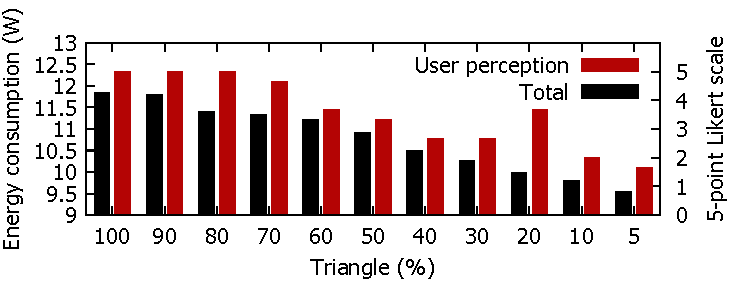
\includegraphics[width=0.8\linewidth]{objectQuality_cropped}
%    \vspace{-2ex}
%    \caption{Power consumption and perception scores for varying object qualities (triangle %usage percentages with respect to original 69K triangle object).}
%    \label{fig:lpgl-optimized}
%\end{figure}

%Next, we validated the effort of different object quality levels on both power consumption and user perception by presenting to our test users 11 different Stanford bunnies -- each  with different triangle counts. \fig\ref{fig:lpgl-optimized} presents the power consumption for each case along with the user perceived quality scores on a 5-point Likert scale. We observed that the power consumption decreased linearly while the user perception was high until after the 70\% mark.  

%Furthermore, given the power consumption reduction-to-usability trade off in %\fig\ref{fig:lpgl-optimized} and qualitative feedback from the study participants %(indicating that quality loss beyond the focal angle was not disturbing), we %select level 1 simplified objects to contain 10\%, and level 2 simplified objects %to contain 5\% of the original triangle 


%This suggests that even if we were to use a reduced triangle object of 70\% of %the original (even for objects in the core focal angle), the users would not know %a significant difference in usability.
%%
%
%we presented nine different 3D objects of varying
%triangle count (object size 1~m in height at 2~m distance) to nine users.
%
%Specifically, the Stanford Bunny that we present has the original number of
%triangles in the 100\% case, but this triangle count decreases by 10-90\%. 
%
%count. 


%
%These results suggest that spending energy to render objects at higher fidelity
%than 70\% of the original will not have a significant impact on the 
%system's usability aspect.
%
%In other words, even if the user is gazing at a specific object (i.e., object 
%is within the core focal angle), we can present a simplified object to conserve
%energy. 
%
%Therefore, we can further optimize the performance of {\myit} using such 
%quality thresholds; 

%\jk{I don't like this statment... but that's what we have...}

%Note that in this experiment we made a small change to the Stanford Bunny so that the bunny had a sphere plugged in to its left eye as in \fig\ref{fig:user-bunny}(c). Four of our five study participants noted that the sphere started to look different 


%%%%%%%%%%%%%%%%%%%%%%%%%%%%%%%%%%%%%%%%%%%%%%%%%%%%%%%%%%%%%%%%%%%%%%%%%%%%%%%%

\subsection{Latency Overhead}

%\begin{figure}[t]
%    \centering
%    \vspace{-2ex}
%    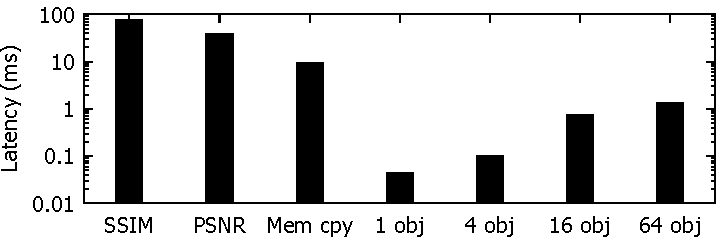
\includegraphics[width=0.8\linewidth]{latency_cropped}
%    \vspace{-2ex}
%    \caption{SSIM, PSNR, and {\myit} Latency}
%    \label{fig:latency}
%\end{figure}

We now analyze the latency of {\myit}, in particular the latency it adds to the rendering pipeline.  We found that the additional latency per-object for {\myit} was 45.57$\mu$sec. As the number of objects increases, the overall latency of {\myit} increases sub-linearly and was $\sim$1.2ms for 32 objects and $\sim$2.5ms for 64 objects. In addition, the latency to perform {\myit}'s run-time object simplification for dynamical loaded objects is 819~msec when simplifying a 69K triangle object to 50\%. This long latency is fortunately a one time process when the object is first used. Later when the object is re-used, {\myit} loads the pre-simplified object to the scene with minimal latency. Overall, the latency of {\myit} is low and does not add any noticeable delay.

%\fig\ref{fig:latency} show the {\myit} latency when  
%1 to 32 objects are presented on the scene. 
%, the overall added latency was still less than 1 ms (as the 
%we see increasing latency, but still noticeably lower than 
%the latency introduced by PSNR and SSIM by multiple orders of magnitude. 


%, and also compare with other frame
%similarity metrics widely used for frame dynamics computation 
%(e.g., SSIM and PSNR).
%
%Note that both SSIM and PSNR are computed for the entire frame as a whole;
%therefore, it does not scale with the number of objects. 
%However, they add the overhead of copying GPU frame buffer contents to the 
%memory for frame dynamics computation. 
%

%
%Specifically, the latency introduced when determining the mesh simplification
%level and culling range is static for any scene, given that these decisions 
%are made based on the mobile device's field of view and the predefined parameters 
%mentioned above. On the other hand, 
%
%This latency will be affected by the number of objects that are displayed
%given that {\myit} operations are dependent on the bounding-box of \textit{each} %object. 
%With more objects, {\myit}'s RDCC would iterate more. 
%

%\fig\ref{fig:latency} and also compare its performance with other frame similarity metrics that are widely used for frame dynamics computation (e.g., SSIM and PSNR). The results show that the overhead from computing the mesh simplification level and culling range is minimal. However, the frame dynamics scoring, as the number of objects increase, the latency increases to a high level. In some cases, with a large number of objects, the {\myit}'s latency exceeds the computation time for SSIM and PSNR. Note that both SSIM and PSNR is computed for the entire frame as a whole; therefore it does not scale with the number of objects in the scene. However, when using SSIM and PSNR for frame dynamics scoring, there is an additional overhead of copying the fram buffer contents from the GPU to the memory for frame dynamics computation. \fig\ref{fig:latency} shows that this additional latency (that occurs on a per-frame basis) is 45.57$\mu$sec for a single object. As the number of objects increase, we see an increase in the latency, but these values are noticeably lower than the overhead introduced by frame image comparison based methods, by three orders of magnitude. 

%Lastly, we present the latency performance of our dynamic scene quantification scheme compared to traditional image comparison methods such as SSIM and PSNR. 

%%%%%%%%%%%%%%%%%%%%%%%%%%%%%%%%%%%%%%%%%%%%%%%%%%%%%%%%%%%%%%%%%%%%%%%%%%%%%%%%

\subsection{Heat Reduction}
\label{sec:heat}


\begin{figure}[t]
    \centering
    \vspace{-1ex}
    \subfigure[Magic Leap One GPU heating]{
        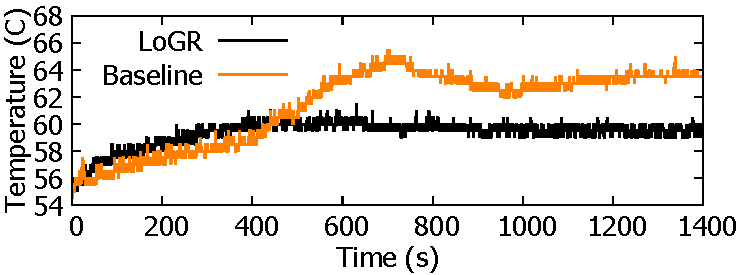
\includegraphics[width=0.46\linewidth]{frame_rate_heat-h_cropped}
        \label{fig:magicleap-heat}
    }
    \subfigure[Magic Leap One frame rate]{
        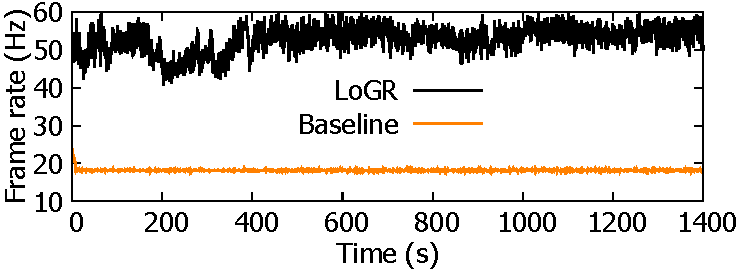
\includegraphics[width=0.46\linewidth]{frame_rate_heat-fr_cropped}
        \label{fig:magicleap-framerate}
    }
    \subfigure[Hololens device heating]{
        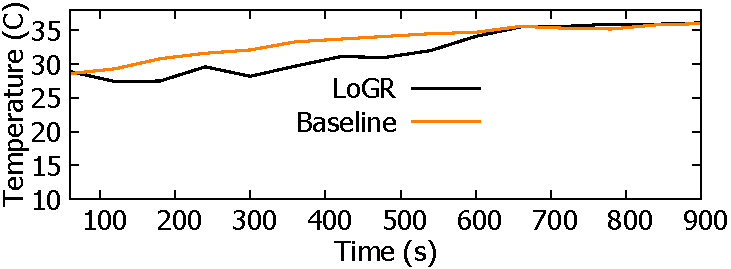
\includegraphics[width=0.46\linewidth]{hololens_heat_cropped}
        \label{fig:hololens-heat}
    }
    \subfigure[Hololens frame rate]{
        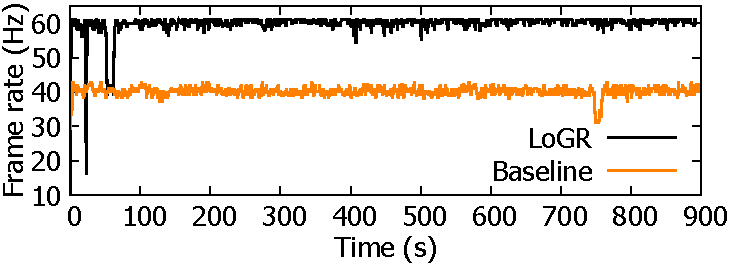
\includegraphics[width=0.46\linewidth]{hololens_frame_rate_cropped}
        \label{fig:hololens-framerate}
    }
    \vspace{-2ex}
    \caption{Temperature and achieved frame rate for the {\mlo} and Microsoft Hololens}
    \label{fig:temp-all}
\end{figure}


%\begin{figure}[t]
%    \centering
%    \vspace{-1ex}
%    \subfigure[Device temperature]{
%       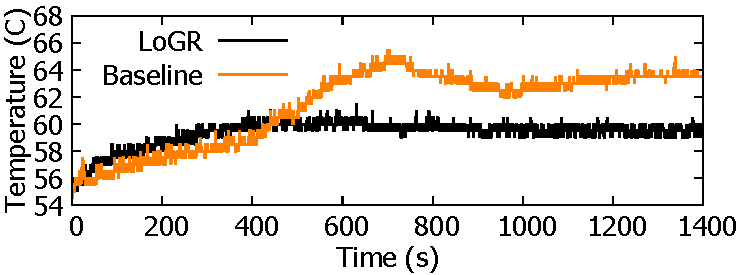
\includegraphics[width=0.46\linewidth]{frame_rate_heat-h_cropped}
%        \label{fig:magicleap-heat}
%    }
%    \subfigure[Achieved frame rate]{
%        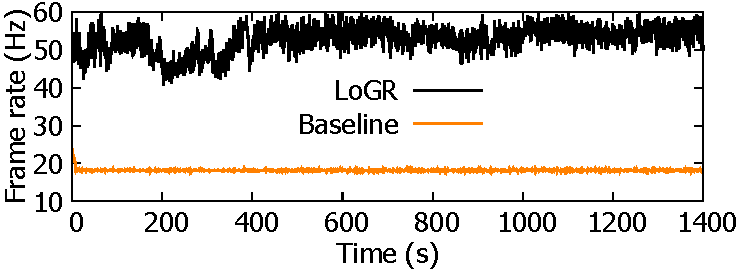
\includegraphics[width=0.46\linewidth]{frame_rate_heat-fr_cropped}
%        \label{fig:magicleap-framerate}
%    }
%    \vspace{-2ex}
%    \caption{Temperature and achieved frame rate for the {\mlo}. \jk{change to baseline}}
%    \label{fig:magicleap-all}
%\end{figure}

%\begin{figure}[t]
%    \centering
%    \vspace{-1ex}
%    \subfigure[Device temperature]{
%       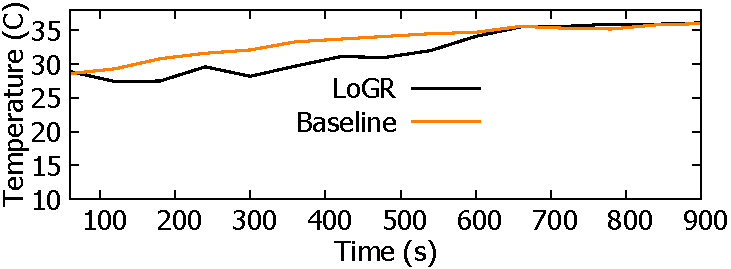
\includegraphics[width=0.46\linewidth]{hololens_heat_cropped}
%        \label{fig:hololens-heat}
%    }
%    \subfigure[Achieved frame rate]{
%        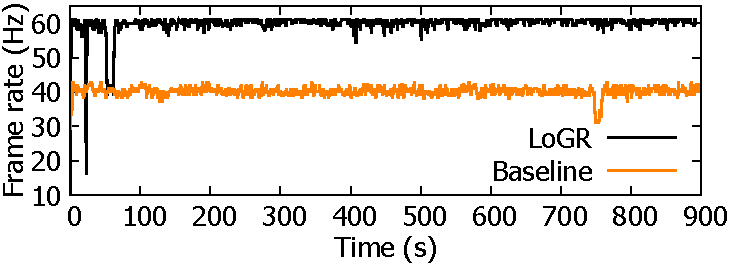
\includegraphics[width=0.46\linewidth]{hololens_frame_rate_cropped}
%        \label{fig:hololens-framerate}
%    }
%    \vspace{-2ex}
%    \caption{Temperature and achieved frame rate for the Microsoft Hololens. \jk{change to baseline}}
%    \label{fig:hololens-all}
%\end{figure}


Finally, we also see device heating as another important factor to consider as mobile AR headsets are worn directly on the head, and high operation temperatures can negatively affect the usability. Therefore, we measure the temperature of the {\mlo} and the Microsoft Hololens with and without applying {\myit} using a dynamic application that saturates the GPU's performance. Specifically, we record how the GPU/device temperature changes over time, along with their achieved frame rates and present the results in \fig\ref{fig:temp-all} for {\mlo} and Hololens. Note that the {\mlo}'s processing units are external to the headset. The users can carry an external processing unit wired to the headset device. On the other hand, on the Hololens, all processing units are integrated to the forehead component of the headset itself. Measuring heat on the {\mlo} was done using its power and thermal profiler and we present the GPU temperature, which dominates the processing unit's temperature. As the Hololens does not provide such analysis software, we used an infrared thermal camera to capture its forehead processing unit temperature on a per-minute basis.


From \fig\ref{fig:magicleap-heat}, we observe that, on the {\mlo}, the GPU temperature of the baseline saturates at a higher level compared to {\myit} and that {\myit}'s achieved frame rate is consistently higher. We see similar patterns for the Hololens (\figs\ref{fig:hololens-heat} and~\ref{fig:hololens-framerate}). 

%Note: the GPU saturates as a similar temperature but achieve a higher frame rate %in general.

%Note: the {\mlo}'s external GPU saturates as a similar temperature as the Hololens but achieve a higher frame rate in general.

%that the device temperature for the two schemes saturate as a similar level, but %differences in frame rates suggest that {\myit} offers higher quality contents %with same amount of heat generation. 


%achieves a high frame rate to tolerate the amount of scene dynamics, the baseline %scheme cannot accommodate for the such dynamics and the frame rate drops to $<$20. 
%
%We conducted this experiment with two device such as magic leap one that we deal with this study mainly and additional hololens. 
%
%

%As shown in the \fig\ref{fig:magicleap-heat}, the temperature of the magic leap one was higher at first when {\myit} was applied, but it did not rise above a certain temperature and maintained at about 60 ° C. When {\myit} was not applied, it rose to 65.5 ° C and maintained at about 63.5 degrees. At this time, in \fig\ref{fig:magicleap-framerate}, the frame rete when {\myit} is applied is going up and down between 50-60, but when it is not applied, it is kept at a little lower than 20. 
%
%This is because the HMD itself artificially lowers the frame rate in order to reduce the heating value. 
%
%In the case of hololens, it is seen that {\myit} is lower than when the heat rise rate is not applied, and the frame rate is also close to 60 when {\myit} is applied similar to magic leap one, but {\myit} is applied If you do not, you can see that it is kept at around 40. As can be seen from the two devices, the application of {\myit} shows that it can maintain a high frame rate while reducing the calorific value.

\section{User Studies}
\label{sec:userstudies}


%%%%%%%%%%%%%%%%%%%%%%%%%%%%%%%%%%%%%%%%%%%%%%%%%%%%%%%%%%%%%%%%%%%%%%%%%%%%%%%%


We now expand our evaluations to a set of IRB-approved user studies. 
%
Here, we analyze the power savings and usability of {\myit} (and each of its features separately) under various scenarios. 
%
For this purpose, we use three types of applications: a static scene app,
a dynamic/interactive scene app, and one where users were given tasks that relate 
to the fidelity of the objects displayed in the scene. Videos of the apps are in \url{http://is.gd/logr\_mobisys}. 
%
Each experiment runs applications using five different configurations in
randomized order for each participant: 
%
(1) with {\myit}, 
(2) with {\myit} culling only, 
(3) with {\myit} frame rate control only, 
(4) with {\myit} mesh simplification only, and 
(5) without {\myit} (the native graphics rendering process). 
%
% The static application, in which we ask the users to observe static (floating)
% objects while rotating their heads, represents an application where {\myit} 
% can benefit the system performance the most. On the other hand, the dynamic 
% application, a simple game in which the users use the controller to pop sphere
% balls that fly towards the user from each side, represents a worst case
% scenario for {\myit} with high motion dynamics and large amounts of head motion.
% Finally, the object fidelity-based task application was designed to confirm that
% using {\myit} does not degrade the detailed fidelity of complex objects 
% while saving energy. 
%
Our user study involved 25 participants (avg.age: 24.6, 10 female) and the 
overall time to complete an experiment (per-user) was $\sim$30~mins with a \$10 
reward. At the end of each stage testing phase, users provided their subjective scores regarding the scene quality on a 5-point \emph{Likert scale} (very poor:1, very good:5).
%, and the energy usage is recorded using the {\mlo} energy profiler.
%
%\jp{'one stage' is per app? or per setting? or per app\&setting?}
%
%Additional values that we present related to the system's performance was 
%logged during the user studies as well. \jp{what other values?}


\begin{figure}[t]
    \centering
    \vspace{-2ex}
    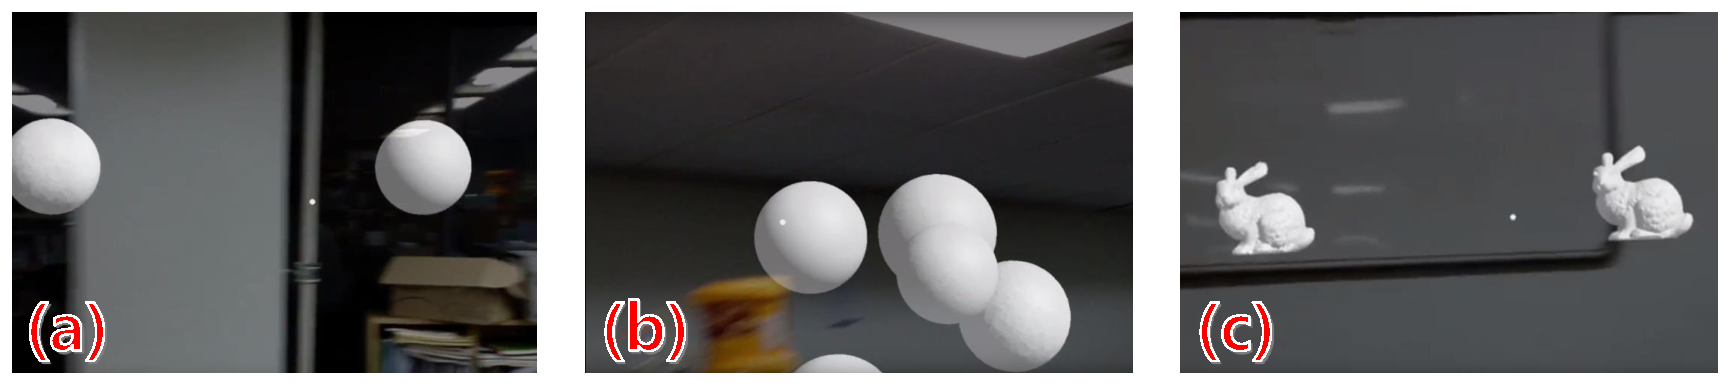
\includegraphics[width=1\linewidth]{scheme2_cropped}
    \vspace{-6ex}
    \caption{Screenshot from our three applications}
%            \jp{please insert some white space (gap) between images}}
    \label{fig:application}
\end{figure}


%%%%%%%%%%%%%%%%%%%%%%%%%%%%%%%%%%%%%%%%%%%%%%%%%%%%%%%%%%%%%%%%%%%%%%%%%%%%%%%%

\subsection{Static Scene App: Floating Spheres}

The purpose of the static scene application (the first app presented to all participants),
was to introduce and familiarize study participants to the mobile AR environment.
%
No specific tasks were given while the users slowly gazed through the 16 spheres
(69K triangles) that float (no dynamics) around the user (equally distributed 
over 360$^\circ$). Each of the five configurations was used for 30 seconds with
short breaks to answer user perception questions after each configuration.


\begin{figure}[t]
    \centering
    \vspace{-2ex}
    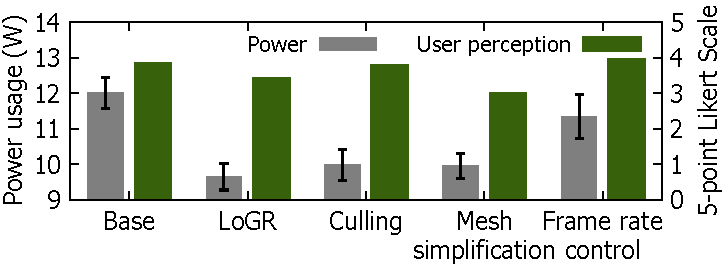
\includegraphics[width=0.8\linewidth]{static_energy_cropped}
    \vspace{-3ex}
    \caption{Mean power usage and user satisfaction scores in 5-point 
            \emph{Likert scale} for static scene app.}
    \label{fig:user-static}
\end{figure}

\fig\ref{fig:user-static} presents the mean power usage and user perception 
results for each test case. 
%
It shows that {\myit} can reduce power consumption by $\sim$22\% ($\sim$2.6~W) 
compared to the baseline graphics rendering process, and the mesh simplification
and culling sub-components contribute heavily to the power savings. 
%
This is because, for the static scene app, the spheres that are not in
the participants' core FOV can be culled or simplified, which leads to 
a significant reduction in GPU and memory usage. From the system lifetime perspective, the results for the baseline translates to 3.0 hours of operation time, and {\myit} adds 0.9 additional hours of operation. 
%

Finally, we can see that the user perceived quality level reports for {\myit} scored 3.54 compared to 3.80 for the baseline, but, this difference was not statistically significant (2-tailed t-test, p<0.05).

%While not significantly different, we explain this difference as the following. In the static scene app, there was no specific task given to the participants, and therefore the they focused closely to the object quality and some were distracted when neighboring spheres were presented in simplified form. This issue is even more prominent when we see the scores for the ``mesh simplification only'' case as well.

%are similar between 3.5-3.9 across all testing configurations.


%%%%%%%%%%%%%%%%%%%%%%%%%%%%%%%%%%%%%%%%%%%%%%%%%%%%%%%%%%%%%%%%%%%%%%%%%%%%%%%%

\subsection{Dynamic Scene App: Sphere Shooting}

The second application is a simple shooting game in which moving spheres fly into the 
scene, and participants are asked to use the controller and
their gaze to ``shoot'' and eliminate the spheres.
%
We design the application so that the spheres to appear in various patterns, in 
high-speeds, low-speeds, from the right and left, etc. %\jp{what kind of bias is this?}
%
Compared to static scenes, this application introduces both dynamics 
and interactive complexity.
%
Again, we test with the five configurations mentioned above and measure the power usage, 
user perception level and the hit/miss rate to quantify task accomplishment levels. 

%The second is a dynamic application like shooting games. This application allows the user to remove the balls coming from left and right sides through the controller. To understand hole energy consumption of that five stage's character, we designed five section in one stage such as default mode, high speed ball mode, low speed ball mode, a lot of balls on the left mode, a lot of balls on the right mode. We asked participants for this study to play the game in 30 seconds.


\begin{figure}[t]
    \centering
    \vspace{-2ex}
    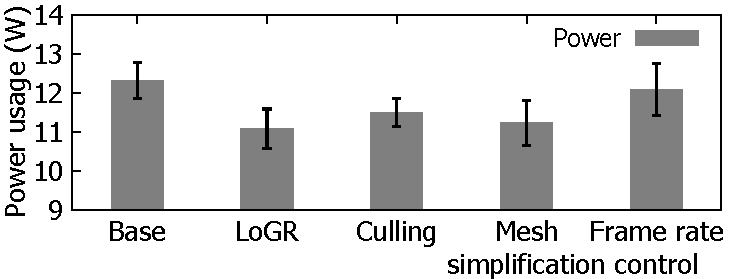
\includegraphics[width=0.75\linewidth]{dynamic_energy_cropped}
    \vspace{-3ex}
    \caption{Mean power usage for dynamic/interactive scene application.}
    \label{fig:user-dynamic-energy}
\end{figure}

%\jp{we are using 'W'... which is a unit of power, not energy.
%we may say 'energy consumption(rate)', but be careful not to say 'energy'}

\fig\ref{fig:user-dynamic-energy} plots the mean power consumption of this 
experiment with standard deviations.
%
Results show that the frame rate component shows only minimal power reduction of 2\%, 
noticeably less than 7\% for the static scene app results in \fig\ref{fig:user-static}. 
%
This is a result of having dynamic scenes, as {\myit} tries to adapt to such 
scenes with high frame rates to preserve application quality.
%
As in the static scene application case, the culling and frame rate control 
plays an important role; as the users focus on the spheres that
they shoot, other spheres can be simplified or culled. Overall, {\myit} 
saves $\sim$11\% power compared to the baseline consumption on average. 


\begin{figure}[t]
    \centering
    \vspace{-2ex}
    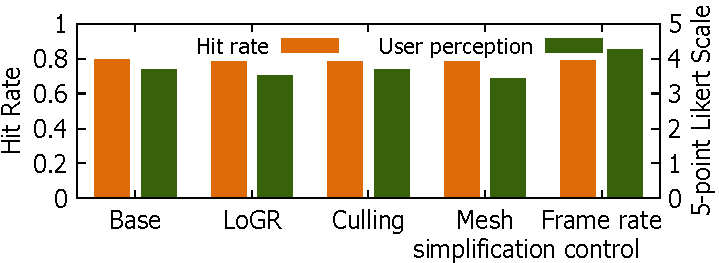
\includegraphics[width=0.85\linewidth]{dynamic_like_hit_cropped}
    \vspace{-2ex}
    \caption{Hit rate and user perception in 5-point Likert scale for dynamic/interactive scene app.}
    \label{fig:user-dynamic-usability}
\end{figure}


In \fig\ref{fig:user-dynamic-usability} we present the mean hit/miss rates 
with the user perception levels. Despite changing the configurations,
there is no noticeable change in the task accomplishment performance 
(i.e., hit rate) and the user perception is kept high across the different test cases.
%
%Compared to the static scene app, in this case, the users were focusing on a more specific task; thus, the small quality degradation did not disturb the quality of executing the target task.

%as well. \jk{potentially add wongyo's comment here}



%%%%%%%%%%%%%%%%%%%%%%%%%%%%%%%%%%%%%%%%%%%%%%%%%%%%%%%%%%%%%%%%%%%%%%%%%%%%%%%%


\subsection{Fidelity-centric App: Bunny Search}


\begin{figure}[t]
    \centering
    %\vspace{-2ex}
    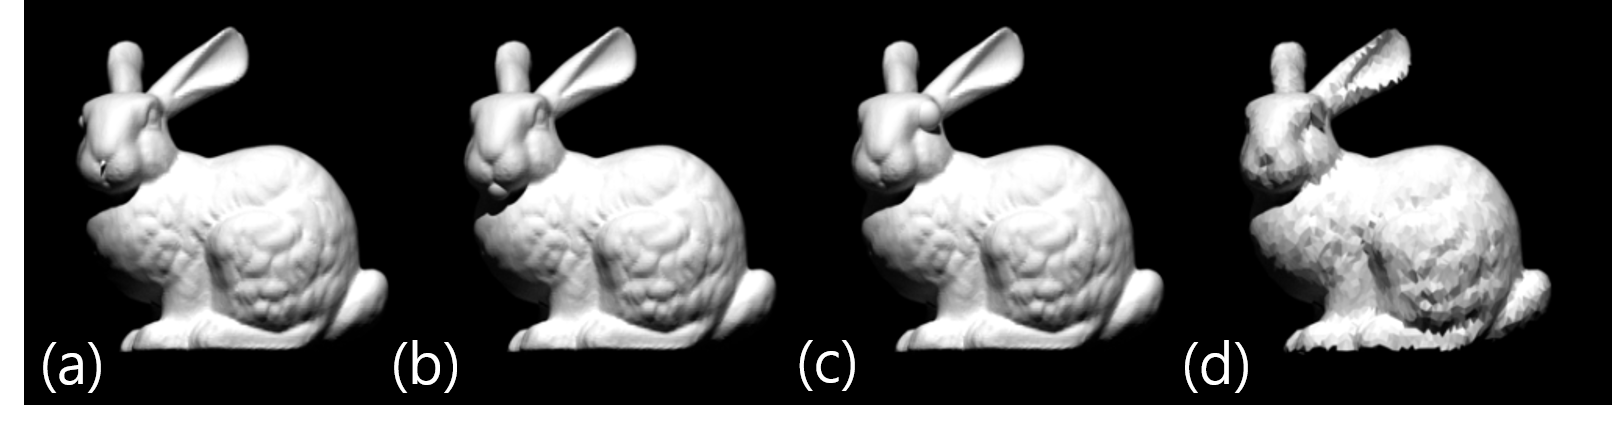
\includegraphics[width=0.9\linewidth]{abnormal_bunnies}
    \vspace{-4ex}
    \caption{Abnormal bunnies designed for our user studies (a)-(c).
            Example of the reduced triangle bunny used for
            the na\"{\i}ve power reduction tests (d).}
    \label{fig:user-bunny}
\end{figure}


The third application used in our user study was designed to conceptualize a group
of real world AR applications in which the fidelity of the displayed object quality 
impacts task accomplishment performance.
%
Specifically, as \fig\ref{fig:user-bunny} shows, we made small, but noticeable,
changes to the original Stanford Bunny by adding small spheres to the eyes or mouth.
%
In the scene, we uniformly distribute 16 bunnies (mixture of normal and abnormal) in 
the 360$^\circ$ space.
%
Study participants would need to look close to the details of each bunny to identify the abnormalities. 
%
We then ask study participants to locate \textit{two} abnormal bunnies with the same 
abnormality. These bunnies are located at least 120$^\circ$ away
from each other to avoid cases where they are adjacent. 
%
We ask for two that are apart (instead of one) to avoid the case where 
an abnormal bunny is located closely at the view point at the beginning of the experiment; 
thus, easy to find with minimal effort.
%
With such scenario, we run three experiments which include 
(1) {\myit}, 
(2) baseline rendering, and 
(3)  na\"{\i}ve power reduction.
%
In the na\"{\i}ve power reduction case, we use the baseline rendering, 
but display bunnies with fewer triangles so that the power usage of the {\mlo}
matches {\myit} (c.f., \fig\ref{fig:user-bunny}).
%
At the beginning of each test, we let the participant know what type of
abnormality they are to find (among the three types), and record the power usage 
and search times until the task successfully completes. Note that prior to performing the three test cases, we allowed the participants to perform one practice run with the baseline rendering mode, so that they well-understood the target task. 


\begin{figure}[t]
    \centering
    \vspace{-2ex}
    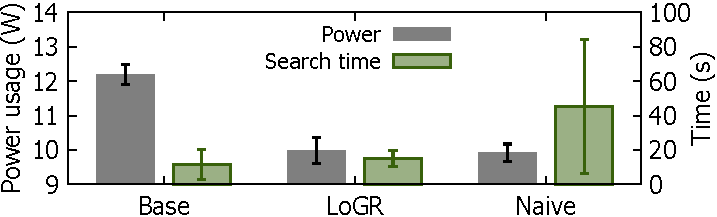
\includegraphics[width=0.8\linewidth]{fidelity_energy_cropped}
    \vspace{-3ex}
    \caption{Mean power consumption and time consumed to accomplish 
            abnormal bunny search task.}
    \label{fig:user-fidelity}
\end{figure}


We present the mean power consumption and the task accomplishment
times in \fig\ref{fig:user-fidelity}.
%
When using {\myit}, we save approximately 20\% in energy compared to the 
baseline. At the same time, the time taken to accomplish the task
was not noticeably affected (11 seconds for baseline 13 seconds for {\myit}).
%
On the other hand, when comparing {\myit} against the 
na\"{\i}ve power reduction case, the power consumption of the two are
similar, but the task completion time differ by more than three-fold.
%
Given that the na\"{\i}ve power reduction case simplifies all displayed 
objects uniformly (see \fig\ref{fig:user-bunny}(d)), identifying the abnormal bunny 
becomes bigger challenge than before, whereas {\myit} reduces power usage while preserving the user perceived scene quality by exploiting the head and gaze orientation data from the mobile headset. 


%The last is a finding bunny that is looking for two bunnies with the features we asked in 16 bunnies. we batched two bunnies with the features because of reducing effect of bunnies space in starting time. For example, when start the game bunnies is located in front of users, the time of game is too short. In this experiments, we wanted to understand different of energy consumption of full {\myit} and no {\myit} and the time it takes to apply bunnies of lower quality to the same application to achieve energy efficiency of {\myit}. 

%\jk{Fig : energy + normalized search time}

%\jk{Fig : show bunny quality using pictures}



%\section{Evaluation}
\label{sec:eval}

%%%%%%%%%%%%%%%%%%%%%%%%%%%%%%%%% 80 CHAR %%%%%%%%%%%%%%%%%%%%%%%%%%%%%%%%%%%%%%

\raj{break this up into lab based detailed power measurements and user study usability results. could be separate sections.}

%valuate the performance of {\myit} using a set of in-lab experiments 
%and an IRB-approved pilot study.

%%%%%%%%%%%%%%%%%%%%%%%%%%%%%%%%% 80 CHAR %%%%%%%%%%%%%%%%%%%%%%%%%%%%%%%%%%%%%%

\subsection{Controlled in-lab experiments}


The goal of our in-lab experiments is to show how each of {\myit}'s components 
contribute to the overall system performance.
%
To evaluate under realistic scenarios, we gathered 12 male and 5 female college
student volunteers to play the block stacking game (Section~\ref{sec:app})
with two modifications.
%
% First, instead of only using box-shaped blocks, our controlled in-lab experiments 
First, instead of using only box-shaped blocks, we
used cylinder-shaped blocks as well in addition to boxes.
%
While boxes are ideal for the purpose of measuring stereoscopsis levels, they 
are not suitable for validating the effectiveness of our mesh simplification
procedure, since a simplified box will still be a box.
%
Second, while the application for patients asks the users to stack five blocks,
we increase this number to 20 for non-patient users.
%
These changes to the application are made so that we have complex enough 
but controllable contents on the screen for fully utilizing and observing the 
benefits that {\myit}'s components offer.


While the volunteers participate,
we record the timestamp, head position, and head direction to formulate a 
``head tracking sample'' $HT_n$ for each participant.
%
Each $HT_n$ is used as a motion trace that we replay to further analyze the 
system-level performance, and in large, we categorized them into two levels of 
head motion; (1) small amount, and (2) large amount of head motions.
%
%\jk{DO WE NEED THIS? 
%Specifically, the position and direction information in $HT_n$ is translated
%to a translation matrix and rotation matrix, respectively.
%We pass the translation matrix through a linear interpolation and 
%the rotation matrix through a spherical linear interpolation to compute 
%the median value and re-position all the objects. 
%By doing so, we can replay the same display contents on the HoloLens 
%without physically moving the device.
%}
%
Using these traces, we analyze how different component and parameters in {\myit}
%such as binary tree-based mesh simplification, quad tree-based dynamics
%scoring, and culling, 
affects the energy usage performance of the HoloLens.


%%%%%%%%%%%%%%%%%%%%%%%%%%%%%%%%% 80 CHAR %%%%%%%%%%%%%%%%%%%%%%%%%%%%%%%%%%%%%%


\begin{figure}
    \centering
    \vspace{-1ex}
    \includegraphics[width=0.8\linewidth]{newMeshSimplificationEnergy}
    \vspace{-2ex}
    % \caption{Impact of binary tree depth $d_B$ on HoloLens energy 
    %         consumption with our block+cylinder stacking application, 
    %         compared with the case without {\myit}.}
    \caption{Impact of binary tree depth $d_B$ on energy 
            consumption compared with the case without {\myit}.}            
    \label{fig:meshsimplification-energy}
\end{figure}


%%%%%%%%%%%%%%%%%%%%%%%%%%%%%%%%% 80 CHAR %%%%%%%%%%%%%%%%%%%%%%%%%%%%%%%%%%%%%%

\spar{Binary Tree-based Mesh Simplification}:
%
We first measure the energy usage rate (mWh/10min) with and without {\myit}.
%
While doing this, we varied the binary tree depth $d_B$ of the mesh 
simplification algorithm to see how much complexity {\myit} can handle.
%
As \fig\ref{fig:meshsimplification-energy} confirms, {\myit} offers an energy
savings of up to $\sim$25\% compared to the case without {\myit}, reducing it
down close to the baseline usage rate ($\sim$490 mWh/10mins) of the 
platform even under minimal workloads.
%
This reduction holds even when a fairly deep binary tree ($d_B$=10) is 
constructed for 20 objects, which implies that our mesh simplification manages
to keep the computation (and energy) costs low.
%
Increasing depth $d_B$ does lead to a slight increase in energy usage since it
results in projecting more ``detailed'' objects, but insignificant up to a 
point where the computational load exceeds what can be handled by
the baseline limit. 
%
After this point, the energy consumption shows a steep increase. 
This is exemplified by a case where we doubled the number of objects on the 
scene (from 20 to 40) with $d_B$=10.

\begin{figure}[t]
    \centering
    \vspace{-2ex}
    \subfigure[Per second average frame rate when varying the frame dynamics 
                threshold for large amounts of motion.]{
        \includegraphics[width=0.8\linewidth]{newFrameDynamicsTraceLarge}
        \label{fig:framedynamics-trace-large}
    }
    \subfigure[Per second average frame rate when varying the frame dynamics 
                threshold for small amounts of motion.]{
        \includegraphics[width=0.8\linewidth]{newFrameDynamicsTraceSmall}
        \label{fig:framedynamics-trace-small}
    }
    \subfigure[Energy savings for varying dynamics thresholds.]{
        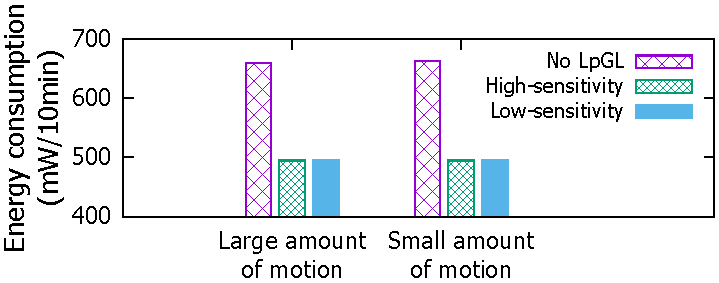
\includegraphics[width=0.8\linewidth]{frameDynamicsEnergy}
        \label{fig:framedynamics-energy}
    }
    \vspace{-2ex}
    \caption{Impact of frame dynamics thresholds on HoloLens frame rate and 
            energy consumption.}
    \label{fig:framedyanmics}
\end{figure}


%%%%%%%%%%%%%%%%%%%%%%%%%%%%%%%%% 80 CHAR %%%%%%%%%%%%%%%%%%%%%%%%%%%%%%%%%%%%%%


\spar{Frame Rate Control and Quad-tree-based Frame Dynamics Scoring}:
%
Next, we examine the impact of QDS on {\myit}'s energy efficiency by monitoring
how the frame rate changes with different target sensitivity thresholds.
%
Sensitivity of frame rate control can be configured using a set of thresholds 
$DT_n (n=1,2,...)$ that determine at what frame dynamics score the frame rate
will shift to a new value.
%
For this experiment, we selected three frame rate levels: 60, 30 and 15 fps.
%
Then, two dynamics score thresholds $DT_1$ and $DT_2$ will determine the frame
rate transitions between 60--30 fps and 30--15 fps, respectively.
%
Note that it is possible to configure frame rates at finer granularity with
more thresholds.
%
For the purpose of our experiments, we set configurations for
``high-sensitivity'' as [$DT_1$=50, $DT_2$=30], and 
``low-sensitivity'' as [$DT_1$=90, $DT_2$=50].
%
For example, with the high sensitive setting, if the frame dynamics score is 
larger than 50, the frame rate is set to 60 fps, and if less than 30, 15 fps is used.
%
%Whereas for the low-sensitivity case, only frame dynamics scores of higher 
%than 90 will put the system in 60 fps mode.
%
%Note that the scope of this work does not include a scheme to personalize or
%adaptively control this threshold, but we leave this as future work. 



\figs\ref{fig:framedynamics-trace-large} and~\ref{fig:framedynamics-trace-small}
plot how {\myit} changes the frame rate over time for large and small amount of 
head motions, respectively.
%
Here, ``High sensitivity'' {\myit} shows a higher frame rate compared to the
``Low sensitivity" case.
%
Furthermore, by comparing \figs\ref{fig:framedynamics-trace-large} 
and~\ref{fig:framedynamics-trace-small}, we can see that since large motions
lead to frequent empty scenes (user moves view away from blocks and
no object motion is detected) the average frame rate stays lower.
%
\fig\ref{fig:framedynamics-energy} again clearly shows that {\myit} reduces 
the energy usage of the HoloLens.
%
However, the difference between the high and low sensitivity cases are negligible
despite the frame rate differences 
(in Figures ~\ref{fig:framedynamics-trace-large} and~\ref{fig:framedynamics-trace-small}).
%
Again, this is due to the HoloLens' baseline energy. That is, {\myit} lowers 
the energy usage down to a point where it cannot be reduced further.


%This shows an example of how the frame rate can change with different sensitivity settings and we now focus on how such changes affect the energy usage performance using different $HT_n$ samples. Specifically, we select one $HT_n$ with large amounts of motion and another sample with a small amount of motion in the data and set the HoloLens to run at different Quad-tree-based Frame Dynamics Scoring sensitivity configurations. Furthermore, we set a mesh simplification depth of 4 for cylinder blocks with \todo{n} triangles and another case with the mesh simplification option off. We measure the the energy usage of the HoloLens under such configurations. As \fig\ref{fig:framedynamics-energy} shows, with the mesh simplification on, regardless of the frame dynamics sensitivity, the HoloLens saves $\sim$25\% of the energy usage, compared to the case where {\myit} is not used. Results also show that with different sensitivity configurations, \jk{Add results!}


%%%%%%%%%%%%%%%%%%%%%%%%%%%%%%%%% 80 CHAR %%%%%%%%%%%%%%%%%%%%%%%%%%%%%%%%%%%%%%


\begin{figure}
    \centering
    \vspace{-2ex}
    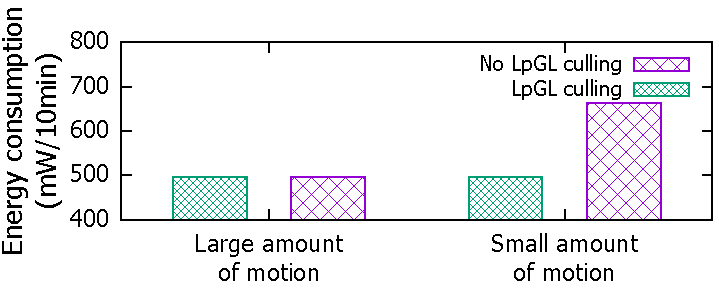
\includegraphics[width=0.8\linewidth]{cullingEnergy}
    \vspace{-2ex}
    \caption{Impact of culling on the HoloLens energy consumption for different head motion samples.}
    \label{fig:culling-energy}
\end{figure}


%%%%%%%%%%%%%%%%%%%%%%%%%%%%%%%%% 80 CHAR %%%%%%%%%%%%%%%%%%%%%%%%%%%%%%%%%%%%%%

\spar{{\myit} Culling}:
%
To verify the impact of {\myit}'s culling on energy, we test with 
and without {\myit}'s culling component turned on. When it is off, only the 
graphics stack's default culling is used. 
%
\fig\ref{fig:culling-energy} shows that, with small amounts of head motion,
{\myit}'s culling feature indeed offers significant ($\sim$27\%) energy savings.
%
In this case, all 20 blocks will be drawn on the scene for most of the time, 
but a subset of the blocks will move out of the FOV
for short periods when the user is moving the blocks.
This is the time when {\myit}'s culling successfully suppresses their 
processing and lowers the energy consumption. 
%
Unexpectedly, however, when there is large amount of head motion, the default 
culling also shows low energy usage rate.
%
This an effect caused by the peculiarity of our application scenario.
Once a user makes large head movements, already stacked 
existing blocks move out of the scene for long periods.
%(similar to the effect in \figs\ref{fig:framedynamics-trace-large} 
%and~\ref{fig:framedynamics-trace-small}). 
%
At this point, due to the simplicity of the scene \rev{(with no backgrounds)}, 
the graphics pipeline is not doing much work even without {\myit}. Therefore, 
both options consume the baseline energy despite {\myit} suppressing tasks up
to the vertex shader.
%
But as the small amount of head motion case shows, {\myit}'s enhanced culling
is beneficial when there are sufficient number of objects in the scene and the
system operates at the boundary of the baseline workload limit.

%%%%%%%%%%%%%%%%%%%%%%%%%%%%%%%%% 80 CHAR %%%%%%%%%%%%%%%%%%%%%%%%%%%%%%%%%%%%%%

\begin{figure}[t]
    \centering
    \vspace{-1ex}
    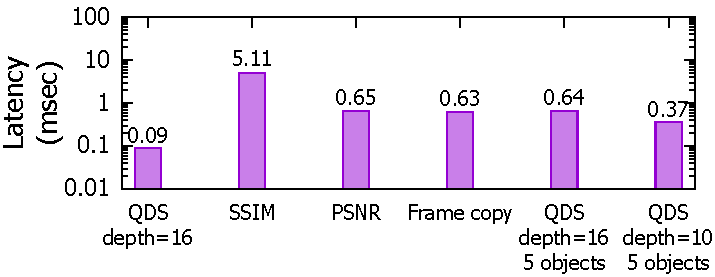
\includegraphics[width=0.8\linewidth]{dynamicScoringLatency}
    \vspace{-2ex}
    \caption{Latency comparisons for different scene dynamics scoring methods
            (Quad-tree based dynamics scoring (QDS), SSIM, and PSNR).}
    \label{fig:dynamicScoringLatency}
\end{figure}

%%%%%%%%%%%%%%%%%%%%%%%%%%%%%%%%% 80 CHAR %%%%%%%%%%%%%%%%%%%%%%%%%%%%%%%%%%%%%%

\subsection{Computational Latency}


An important factor we should consider besides energy is the latency of the 
algorithms we've designed in {\myit}. If algorithms take long to execute, 
this too can affect the user experience and disrupt application requirements.
%
\fig\ref{fig:dynamicScoringLatency} plots the latencies for computing the 
screen dynamics using various methods. Our scheme, QDS, is compared with 
widely used image-based frame dynamics computing methods such as SSIM and PSNR.
%
To compute at the same granularity, we set $d_Q$ as 16. Here we use a scene 
which consists of a cube in the center. Comparing the first three bars show 
that the latency of QDS-based frame dynamics computation ($\sim90~\mu$sec per frame)
is significantly lower than the SSIM ($\sim$55x) and PSNR ($\sim$7x).
%
The fourth bar, in which we plot the time spent by the PSNR and SSIM schemes 
while copying the frame buffer contents from the GPU to the memory for dynamics 
computation, shows that a large portion of this latency (the majority for 
PSNR; 0.63 of 0.65 msec) is wasted on the memory copy process.
%
This result suggests that our geometry-based approach can
outperform the image-based algorithms. It is especially true for
AR HMDs given that only a small portion of the scene is usually drawn
on the screen compared to VR or mobile AR applications. 


Next, we try adding four additional cubes to the scene and compute the latency
for QDS. The fifth bar in \fig\ref{fig:dynamicScoringLatency} shows that when
more quad trees are constructed to support more objects, the latency of QDS 
increases rapidly.
Nevertheless, from the sixth bar we can see that lowering $d_Q$ to 10 (from 16)
shows a much decreased latency of 0.37 msec.

\begin{figure}[t]
    \centering
    \vspace{-1ex}
    \subfigure[Binary tree construction latency for varying tree depths]{
        \includegraphics[width=0.41\linewidth]{octreeLatency}
        \label{fig:octree-latency}
    }
    \hfill
    \subfigure[Simplified Stanford Bunnies using binary tree-based mesh simplification]{
        \includegraphics[width=0.39\linewidth]{simplifiedBunnies}
        \label{fig:octree-bunny}
    }
    \vspace{-2ex}
    \caption{Binary tree construction latency for Stanford Bunny and 
        the results of mesh simplification.}
    \label{fig:octreeConstructionLatency}
\end{figure}

%\begin{figure}[t]
%    \centering
%    %\includegraphics[width=1\linewidth]{}
%    \caption{The simplified bunny 3D models}
%    \label{fig:simplifiedBunnies}
%\end{figure}

The latency introduced by the binary tree construction process is presented in 
\fig\ref{fig:octree-latency} for the full-resolution Stanford Bunny with 
$\sim$69K triangles while varying $d_B$.
%
We also present the outcome of the binary tree-based mesh simplification in 
\fig\ref{fig:octree-bunny} for different depths. Results show that the mesh 
simplification process for a full-resolution Stanford Bunny takes less than 
$\sim$80~msec for $d_B\le$11 and the latency converges (at $\sim$140~msec) for 
higher $d_B$ values.
%
Given that these simplified objects will be displayed for objects that are 
\textit{out of} the user's focus range (by more than $\epsilon^\circ$) we can 
see that voxelization effectively simplifies the target objects.
%
%Note that  given the binary tree depth of $d_B$ and $n$ triangles,
%the theoretical complexity is $O((2n)^{d_B})$. Nevertheless, at each step
%{\myit} only checks for vertex inclusions in the binary tree; thus, the
%quantitative results are small enough to induce minimal effect on the user
%experienced latency. 


%%%%%%%%%%%%%%%%%%%%%%%%%%%!!DO NOT USE!!!!%%%%%%%%%%%%%%%%%%%%%%%%%%%%%%%%%%%%%
%%%%%%%%%%%%%%%%%%%%%%%%%%%!!DO NOT USE!!!!%%%%%%%%%%%%%%%%%%%%%%%%%%%%%%%%%%%%%
% 먼저 우리는 환아를 대상으로 실험을 진행하기 전, 20대 30대 성인 남녀 x 명을 대상으로 사전 실험을 진행했다.
% 이번 실험에서는 설문을 더 잘 이해할 수 있는 성인들을 대상으로 Block stacking 실험을 진행하여 Strabismus Patients 환아 들에게 적용할 실험의 feasibility를 알아보았고 {\myit} 적용으로 인해 발생하는 퀄리티 저하에 대해 미리 알아보기 위하여 간단한 survey를 진행했다.
% 실험의 protocol은 다음과 같았다. 먼저 block stacking 게임을 실행 시킨 뒤, 조작법을 가르쳐 주어 AR 환경에서의 조작에 익숙해 질 수 있도록 했다. 그 후 세 번의 실험 인스턴스를 수행했다. 하나는 {\myit}를 적용하지 않은 게임, {\myit}를 적용하되 quad-tree dynamics scoring에 대해 높은 감도에서 반응하는 게임, 마지막으로 {\myit}를 적용하되 quad-tree dynamics scoring에 대해 낮은 감도에서 반응하는 게임이었다. 만약 감도가 낮다면 dynamic score가 굉장히 높아야지만 반응하게 되므로 에너지 소모는 아낄 수 있지만 사용자 경험을 희생하게 된다. 반대로 감도가 높다면 조금만 움직이더라도 framerate이 높아져 사용자 경험에는 좋지만 에너지 소모를 줄일 수 있는 가능성은 낮아진다.
% 각 instance를 마친 뒤 우리는 사용자 경험에 대한 설문을 진행했다. 설문의 내용은 다음과 같았다. 1) 눈이 아프지는 않았는가? 2) 불편한 정도를 점수로 나타내면? 3) 어지러움을 느꼈나? 4) 보이는 그림이 뚜렷했나? 5) 화면이 부드러웠나?
% 결과는 다음과 같았다. 먼저, 대부분의 피실험자들이 눈의 고통이나 어지러움을 느끼지 못했다. 불편함에 대해서는 화면의 quality 저하가 영향을 주기보다는 constant하게 AR HMD 환경 자체에 불편함을 느끼는 사람들이 x%였다. 또한 일부 집단은 framerate의 변화에 따른 화면의 부드러움 변화를 인지했지만, 의미있는 다수가 이러한 변화를 인지하지 못했다.
% 이러한 실험을 통해서 우리는 {\myit}가 사용자 경험에 critical한 영향을 주는 것은 아니라고 결론을 내릴 수 있다. //먼저, 대부분의 피실험자이 감도에 상관없이 비슷한 대답을 했다는 것을 알 수 있었다. 수치적으로 보면 (1), (2)번 질문에서는 거의 유사한 대답얻을 수 있었고, (3)번 질문에 대해서는 아주 조금 높지만 마찬가지로 거의 유사한 1.5~2정도 사이의 대답을 얻을수 있었다. 심지어 어떤 case에서는 낮은 감도에서 오히러 더 물체가 또렸하게 보였다는 대답을얻었다.어 을 수 있 심지어 낮은 감도에서 보이는 그림이 더 뚜렷했다고 대답을 한 경우도 있었다. 따라서 우리는 이정도 감도의 변화는피 실험자들의 사용성에 영향을 주지 않는다는 결론을 내릴 수 있었다.
%%%%%%%%%%%%%%%%%%%%%%%%%%%%%%%%%%%%%%%%%%%%%%%%%%%%%%%%%%%%%%%%%%%%%%%%%%%%%%%%
%%%%%%%%%%%%%%%%%%%%%%%%%%%%%%%%%%%%%%%%%%%%%%%%%%%%%%%%%%%%%%%%%%%%%%%%%%%%%%%%

\subsection{3D Block Stacking Application}
\label{sec:app}

%%%%%%%%%%%%%%%%%%%%%%%%%%%%%%%%% 80 CHAR %%%%%%%%%%%%%%%%%%%%%%%%%%%%%%%%%%%%%%

\raj{merge this into the evaluation section for the user study}

To evaluate the usability of {\myit} on a real application at the user level,
we designed an AR application for implicitly measuring the stereoscopsis level 
of children with strabismus using AR HMDs, and performed an Institutional Review
Board (IRB)-approved pilot study with strabismus (i.e., crossed eye) patients in
the ophthalmology department at a university hospital.
%
The purpose of our pilot study was to validate changes in user-perceived
object rendering quality when applying {\myit} with different configurations.


Traditionally, devices such as keratometers are used to measure the 
stereoscopsis level. However, these devices are bulky and cannot effectively 
gain the attention of children to focus during the measurements.
%
For this reason, the clinical staff asked for a more interactive and engaging 
game to measure children's stereoscopsis levels, and we designed an AR-based 
game where the children were asked to stack 3D blocks using Microsoft HoloLens%
\footnote{We used DirectX as the underlying native graphics library}
(c.f., \fig\ref{fig:hololens}).


The block stacking game operates as follows.
%
When the application starts, a white cube palette is displayed.
Once the user visually focuses on the cube, the user is asked to press a clicker
device and move the object in the 3D space.
%
Using such movements, the user is asked to stack all cube blocks on the display.
The performance of moving the objects becomes an indirect measure of the 
stereoscopsis level. 
%
We designed this game and user study to confirm if {\myit} makes proper 
transitions in frame rate or changes in object quality, while minimally 
affecting the user perceived quality.
%
Furthermore, we also gathered statistics on the amount of energy 
that can be saved by applying {\myit} to real-world applications%
\footnote{A sample video of the application and its interaction with {\myit} is
available, and we will provide the URL after the anonymous review process.
%at \todo{http://}
}.

%\jk{Let's make a recording of the task and share on Youtube.}



%%%%%%%%%%%%%%%%%%%%%%%%%%%%%%%%%%%%%%%%%%%%%%%%%%%%%%%%%%%%%%%%%%%%%%%%%%%%%%%%%


% 이러한 실제 stereoscopsis의 측정에 앞서, 우리는 AR HMD의 사용성에 대해서 면밀히 검토할 필요가 있었다. 특히 우리의 실험 대상은 어린이 환자들이었고, 이러한 환자들이 새로운 환경인 HMD 환경을 쉽게 이용할 수 있는지는 큰 챌린지 중 하나였다. 구체적으로 살펴보면 첫번째로 조작의 편의성을 확인해야 했다. Microsoft HoloLens로 조작할 수 있는 주요 방법은 손가락을 통한 gesture 인식과 external 장비인 clicker 가 있다. gesture 인식의 경우 HoloLens에 부착되어 있는 depth sensor에 손이 보여야 하는 문제가 있고 클릭의 정밀도가 낮다는 단점이 있는 반면, clicker를 이용하면 click 이라는 액션이 명확하다는 장점이 있기 때문에 우리는 clicker를 사용하기로 했다. 두번째로 HMD라는 경험이 환자들에게 어떻게 느껴지는지 인 지점이 있었다. 알려져 있기로 HMD 경험이 눈의 고통을 주기도 하고, 어지러움을 야기할 수도 있고, 불편함을 주기도 했는데 실제로 어린이 환자에게 AR 응용을 적용됐을 때 어떤 경험을 주는지 확인해 보는 것은 추후 AR 응용을 개발하는데에 좋은 information이 될 수 있다.  마지막으로 어린이 환자를 위한 측정 방법과 설문의 난이도를 고려하는 것이 중요했다. block stacking이라는 간단한 동작이지만 이러한 동작이 어린이들, 특히 환아들에게 어려울 수 있고 이러한 과정에 대한 설문을 하는 과정도 쉬운 언어를 통해서 진행이 되어야 했다.

%%%%%%%%%%%%%%%%%%%%%%%%%%%%%%%%% 80 CHAR %%%%%%%%%%%%%%%%%%%%%%%%%%%%%%%%%%%%%%

%\subsection{Application-level View Frustum Culling}

% 이번 섹션에서는 draw call을 줄이기 위한 방법인 user level view frustum culling의 방법에 대해 구체적으로 설명한다. 이전 섹션에 말했 듯, culling은 visibility를 판단하는 작업이다. 그래픽스 파이프라인에서는 view frustum culling이라고 불리는 작업을 수행하는데, 이는 카메라 정보, 그 중에서도 종횡비 시야각, 그리고 최소 가시거리, 최대 가시거리 정보를 통해 frustum을 만들고, 렌더링하는 물체들이 frustum의 바깥으로 나가는지 그렇지 않은지를 판단하는 방법들이다. 이러한 방법을 통해 화면에 보이지 않는 triangles를 판단하고, 이후 pipeline 작업에서는 해당 triangles를 배제해서 성능 향상을 이룬다.

% 하지만 그럼에도 불구하고 system level이 아닌 application level에서의 view frustum culling은 필요하다. 그 이유는 렌더링 되지 않는 draw call도 에너지 소모에 영향을 주기 때문이다. 그 이유는 view frustum culling이 일어나는 시점의 문제에 있다. draw call이 불리면 graphics pipeline은 모든 그려야 하는 vertices를 vertex shader를 통해서 병렬적으로 transformation한다. 이 이후 시점에서 view frustum culling이 일어난다. 즉, 실제로 그려지게 될지 모르는 상태에서 연산을 해야 한다는 것이다. 이로 인해 높은 the number of triangles를 가진 모델의 경우 자원을 크게 낭비하게 된다.

% 우리는 다음과 같은 방법을 통해 user level에서 light-weight view frustum culling을 진행한다. gpu에서의 view frustum culling은 mesh의 모든 triangles에 대해서 진행되기 때문에 비용이 비싸다. 하지만 우리는 우리는 mesh의 triangles가 아닌 initialization 시에 만든 mesh의 bounding box를 이용한다. 이러한 bounding box는 모델의 전체를 bound하고 있기 때문에 만약 camera가 바라보고 있는 방향기준으로 시야각 바깥에 bounding box가 있다면 이 모델이 보일 가능성이 없다고 생각할 수 있다. 이러한 케이스에 대해서는 해당 모델에 대한 draw call을 호출하지 않음으로 인해서 에너지 소모를 줄일 수 있다.


%%%%%%%%%%%%%%%%%%%%%%%%%%%%%%%%% 80 CHAR %%%%%%%%%%%%%%%%%%%%%%%%%%%%%%%%%%%%%%

\begin{comment}

To explain the implementation details of the bounding box projection process, we take as example, once again, the Stanford Bunny. Say that there is a Stanford Bunny and we want to compute the three metrics (i.e., XXX, XXX, and XXX) discussed above. Given the vertices and topology information for the bunny rendering, we receive the transformation matrix from the application to apply the target transformation (e.g., scaling, rotation, translation) to the vertices. On the application's perspective, as a result of the transformation process, a vertex $V$ will be located at $(x,y,z)$ from the origin point $(0,0,0)$. Here we say that $V$ is transformed in to world-space. \jk{huh???}

% 간단한 예로 화면에 stanford bunny가 그려져 있고, 우리가 위에서 정의한 세가지 방법들을 계산하기 위해 유저 입장에서 이 bunny가 어떻게 보이는지를 계산하고 싶다. 렌더링을 하기 위한 vertices와 topology information이 있을 때, 이에 원하는 transformation (e.g. scaling, rotation, translation)을 적용하기 위해 transformation matrix를 application 단으로부터 받아서 vertices에 곱해준다. 이렇게 transform된 vertices는 중 하나의 vertices v 는 application 입장에서 origin, 즉 (0, 0, 0)을 기준으로 (x, y, z)에 위치하게 된다. 이때의 v를 v is transformed into world space. 라고 표현한다. 이 상태에서는 user 의 

\end{comment}





\subsection{Pilot Study with Strabismus Patients}
\label{sec:pilot-study}

Finally, using the application discussed in Section~\ref{sec:app}, we performed 
an IRB-approved pilot study with a total of eight children participants 
(ages 7-10), of which four were diagnosed with strabismus and the other four 
visited the hospital for post-surgical check ups.
%
The purpose of this study was to validate changes in user-perceived object
rendering quality (including user experience) when applying {\myit} with different target quality levels.
%
%\rev{and also to verify that applying {\myit} did not disturb the user experience within the application.}


We started our study by teaching the children how to play the block stacking 
game, and had them get used to controlling objects in the AR environment.
%
In the actual experiment phase, we had each child play three versions of the
block stacking application: one version without {\myit}, {\myit} with 
low-sensitivity QDS thresholds, and {\myit} with high-sensitivity QDS thresholds.
%
This information was not disclosed to the participants and the testing order was
randomized to remove any bias.


% Note that the contents of this game is very simple;
% therefore, there is only a minimal amount of energy savings from the frame rate
% control and mesh simplification. Rather than analyzing the energy usage,
% the purpose was to verify that applying {\myit} did not disturb the user 
% experience within the application context.
%
Using a visual analogue scale (VAS) type of survey (1-5 scale), we collected 
information on (1) whether the participant felt any dizziness, (2) the clarity 
of the blocks, and (3) how comfortable the game was to the eyes.
%
We note that all participants responded with answers of similar patterns
regardless of the test scenario.
%
Quantitatively, for questions (1) and (3), most participants answered with 
a score of 1, indicating that the system was comfortable and there were no 
dizziness. Answers for question (2) were in the range of 1.5-2, suggesting that
the clarity was not perfect but acceptable. Surprisingly, some participants 
answered that {\myit} with low-sensitivity showed the most clear images.
Given that we randomized the experiment sequence, this suggests that frame 
rate changes (for our application) gave minimal effect to the
usability and object quality.


\rev{
We acknowledge that eight children participants are not a large enough and
representative user population to generalize our user study given the broad 
range of AR applications.
%
However, they are unbiased, and we emphasize that the study was performed 
for a real use case at the hospital.
%
We plan to extend our case study to a more diverse set of applications with
larger subjects as part of our future work.
}


%%%%%%%%%%%%%%%%%%%%%%%%%%%%%%%%% 80 CHAR %%%%%%%%%%%%%%%%%%%%%%%%%%%%%%%%%%%%%%



\section{Discussions and Future Work}

%Based on our experience, we outline several interesting points for 
%further discussion and needing future investigation.

%In this work, we defined scene dynamics metric as the maximum speed of visible objects, which is faster then image-based method(e.g. PSNR) and granularity-free.
%To realize geometry-based method, the underlying system should be able to access transformation information of objects. {\myit} can capture transformation by Front-end API without any additional overhead.
%However geometry-based dynamics scoring cannot work for image based application like 360$\circ$ video streaming application.

\spar{Applicability to other mobile AR headsets:}
%
{\myit} is designed to be a device and platform-independent solution for reducing power usage on mobile AR headsets. Given that its design is centered around the standard graphics pipeline and native graphics library APIs (e.g., OpenGL), the implementation is easy to port for different platforms. In this work, while we mostly focus on the performance statistics of the {\mlo}, as the results in Section~\ref{sec:heat} shows, {\myit} is already implemented for use on the Microsoft Hololens as well. We note that we observed similar power usage reduction patterns on the Hololens by saving $\sim25\%$ of power for static scenes and $\sim12\%$ for dynamic scene applications. As part of our future work, we plan to expand {\myit} support for different mobile AR platforms as well.

%Furthermore, since {\myit} focuses on object characteristics, while designed for AR apps, we see potential in applying similar techniques to VR headsets as well.

% this is where either we have already shown it with Hololens results or we give some Hololens results. -- emphasize that this scheme is generally applicable...

%{\myit} is applicable to other another AR headsets like Microsoft HoloLens. We implemented {\myit} on HoloLens and conducted energy consumption measurement on static scene scenario aforementioned. As similar with Magic Leap One, {\myit} could save x\% of power consumption of HoloLens as well.
%
%{\myit} is portable to graphics-based platform by reason of its minimal assumption. {\myit} requires only standard graphics pipeline and the most of modern mobile platform which have display and GPU provides graphics API like OpenGL or DirectX. By this characteristic {\myit} might be portable to general mobile phone or VR devices, but there should be preceded investigation on energy consuming characteristic of each devices.

\spar{Power management of headset and other components:}
%
While our preliminary studies show that the headset itself is also a major consumer of power, this work focuses on the graphics pipeline-related aspects of mobile untethered AR platforms. Techniques such as those that duty-cycle the headset sensors and adaptively control the brightness/resolution of objects, combined with our efforts in optimizing the graphics pipeline, can have significant impact in increasing the lifetime of mobile AR headsets. However, the fact that the {\mlo}, along with many other commercially available mobile AR headsets, expose only limited access to the headset configurations limits such research at this point. 

In addition, the power usage of components such as WiFi need to be collectively managed. As mentioned in Section~\ref{sec:preliminary}, findings from many previous work~\cite{Qian2018, Qian2018TVP, Abari2017} can be applied to reduce WiFi power usage in mobile AR applications. Overall, we see this as an interesting direction of research towards designing a comprehensive framework for mobile AR headset power management. 


\spar{User study limitations: }
%
Given that mobile AR headset development is still in its early stages, real-world applications for exploiting these platforms' full capabilities are still premature. At the same time, considering the impact that these new wearable computing devices can offer, the domains in which they can potentially contribute to can become very diverse. For this reason, while we wanted to test {\myit} on a real-world, widely used application, it was difficult to define a single set of applications that were representative for mobile AR headsets. For this reason, our user studies focus on three types of applications, each with different application and scene characteristics. We do so to make sure that our evaluations cover diverse cases in how mobile AR headsets can contribute in novel applications. Nevertheless, the performance of {\myit} and untethered mobile AR headsets in general will heavily depend on application complexity and its requirements, and we hope to apply {\myit} on real-world applications as part of our future work.

%\spar{Additional Improvements:}
%
%A core feature of {\myit}, frame rate control, is activated using the scene dynamics score computed based on the maximum speed of objects moving on the scene. While effective, there are limitations. Given our scheme focuses on the ``movements'' computed using the bounding-box of the object (to minimize computational complexity), if for example a sphere-shaped globe was to rotate 360$^\circ$ without coordinate changes, {\myit} would not be able to capture such dynamics. This is a fundamental limitation of geometry-based schemes that compute the scene dynamics and as part of future work we plan to explore additional scene dynamics computing methods. 

%On the system's perspective, along with the technologies presented in this work, other power consuming components, such as the display and WiFi. As briefly mentioned in Section~\ref{sec:prelim}, the omit the control of these components due to either the limitations in hardware configurations or 






%We perform our user studies with three different types of applications to show the effectiveness of {\myit} in diverse scenarios. However, g

%In designing user studies, it was hard that defining ``realistic'' and ``representative'' application of AR headset. 1) \textit{pre-maturity of ecosystem} Since AR headsets and their applications are not yet adopted to common users,  2) \textit{Generality}

%Not yet AR headset application ecosystem is not mature

%AR application boundary is too broad.

%\jw{Should include consideration for people who have bad sight.}

% \spar{Power Management Impact on Heat and Comfort}

% The most of participants complained that the heat of headset and it is potentially able to cause user experience quality degradation.
% Unfortunately, the Power and Thermal Analyzer, which is provided by Maigc Leap~\cite{}, does give the temperatures of each components in the board (e.g. CPU, GPU, SoC and so on), but not offer the heat information of the headset.

\begin{comment}
%
{\myit} uses quad-tree-based dynamics scoring method. 
%
Evaluation results suggest that this scheme is energy efficient for screen
contents with a limited number of 3D objects to display.
%
Compared to traditionally widely-used methods such as PSNR and SSIM which
require the entire frame buffer content, our scheme which uses only the 
geometric information is appealing.
%
However, %our results also suggest that a complex display content can result in
%high computational \emph{latency} as well.
%
while the PSNR and SSIM methods can have constant overhead, our scheme's 
\emph{latency} will scale with the number of objects on the scene.
This suggests the need for identifying the limit up to which our scheme can 
benefit over PSNR or SSIM.
\end{comment}
% \jk{limitation of geometry-based schemes is that we cannot capture changes in color/texture for non-moving objects}
%
%Furthermore, because our scheme uses the difference in bounding box coverage
%rather than the actual content when determining the changes in 
%consecutive frames, if in the unlikely case a new object is plotted in the 
%\textit{same} bounding box, the quad-tree-based scheme will not be able to 
%catch this information. We find this case very unlikely and small changes in
%the bounding box can be captured using a deep enough tree. Nevertheless,
%these are remaining issues that we see as important. 



\begin{comment}
\spar{Parameter Tuning}:
%
%Our current version of {\myit} implementation does not provide support for 
Our current version of {\myit} does not provide support for 
optimizing the parameters for a given objective.
%
Hence, we leave the ``freedom'' of configuring the parameters to the
application at the cost of demanding some level of developer involvement.
%
However, to fully achieve transparency with the application, there is a need
for {\myit} to independently understand the requirements of the application 
and also (potentially) its users.
%
On the application perspective, we are performing additional research on 
the requirement set and in the process of identifying a small number of 
preset values that satisfies such requirements.
%
On a per-user adaptation perspective, there is a need to expand user studies
to identify the diverse (minimum) quality requirements of different users.
%Through this process, there is a need to understand how {\myit} can easily
%and quickly adapt to user requirements with minimal training.
%
Indeed, the user and application requirements for parameter settings will be
a combination factor and further studies are needed to achieve the goal of
adaptive parameter auto-adjustment or simplification.



\spar{Closed System}:
%

\raj{this might be unnecessary}

Finally, we had a practical challenge of Microsoft HoloLens being closed. 
This tightly limits the services that third-party developers can provide.
%
First, HoloLens applications are sandbox-based; thus, cannot access the 
system-related information freely. In addition, the lack of internal 
inter-process communication mechanism in UWP limits the development freedom 
and the scope of services that can be designed.
%
Second, all third-party programs are considered as ``applications".
As a result, services such as {\myit} cannot run as background daemons. % or services.
Instead, we had to design {\myit} %so that the implementation stays 
close to the application layer. 
If potentially there are many applications 
interconnected with {\myit}, executing as a daemon service can be beneficial. 
%For example, LiKamWa et al.~\cite{LiKamWa:2015:SEC:2742647.2742663} also proposed a
%dedicated process for vision processing to reduce Google Glass' computation
%load. However, in closed systems, such scheme cannot be directly applied.
%
Finally, head orientation and the view matrix is (currently) the only 
type of fine-grained and real-time sensory information that we can utilize 
from the HoloLens. Despite having depth and temperature sensors on-board,
UWP does not allow applications to access their data. With more sensory data, 
there are potentials to monitor and manage the energy usage in different 
dimensions.

\end{comment}


%%%%%%%%%%%%%%%%%%%%%%%%%%%%%%%%% 80 CHAR %%%%%%%%%%%%%%%%%%%%%%%%%%%%%%%%%%%%%%



%%%%%%%%%%%%%%%%%%%%%%%%%%%!!DO NOT USE!!!!%%%%%%%%%%%%%%%%%%%%%%%%%%%%%%%%%%%%%
%%%%%%%%%%%%%%%%%%%%%%%%%%%!!DO NOT USE!!!!%%%%%%%%%%%%%%%%%%%%%%%%%%%%%%%%%%%%%

\begin{comment}

Statistics on the head direction data is as follows. The average task completion time was X $\pm$ y sec, the average change in head direction was X $\pm$ y \jk{$^\circ$/sec}, and \jk{mW and MW????}. \jw{It was just variable name. I changed it to a and b}
%Among these samples, we select to most active 25\% and the least active 25\% samples for our evaluations. \jk{Why these samples? Average is less meaningful? Extreme is better?}
% 먼저 우리는 head direction data들을 통계 내보았다. 평균적인 작업의 완료 시간은 x +- e초 걸렸고, 평균적인 head direction 변화 속도는 x+-e, 최대 폭과 최소 폭은 각각 a, b였다. 우리는 이 중에서 상위 25% 넓게 움직인 샘플, 하위 25% 조금 움직인 샘플을 골라서 에너지 소모를 측정했다. %{jw: 재생 속도를 조정하는 실험은 시간이 허락하면 진행해야 할 것 같습니다.} 재생 속도를 조정해 각각의 속도를 빠르게 /  느리게 조정하여 에너지 소모를 측정했다.

\begin{figure}[t]
    \centering
    \subfigure[Changes in frame rate when varying the frame dynamics threshold. \jk{Is this a trace??}]{
        \includegraphics[width=0.44\linewidth]{empty}
        \label{fig:framedynamics-trace}
    }
    \subfigure[Energy savings for varying dynamics thresholds.]{
        \includegraphics[width=0.44\linewidth]{empty}
        \label{fig:framedynamics-energy}
    }
    \caption{Impact of the frame dynamics threshold on the frame rate and energy usage of the HoloLens.}
    \label{fig:framedyanmics}
\end{figure}


First, we present in Figure~\ref{fig:framedynamics-trace} on how the frame rate adaptively changes with respect to the changes in the frame dynamics threshold. In Section~\ref{} we mentioned that {\myit} measures the frame dynamics score and the RDCC engine makes decisions on the frame rate of the target object. The threshold ... \jk{Did we ever say what the ``dynamics threshold" is? VERY CONFUSING...} As \fig\ref{fig:framedynamics-trace} shows, for sensitive thresholds, RDCC maintains a high frame rate of 60 fps for ... \jk{WTF.... what does a ``sensitive" threshold mean??? Where do we define this?!?!?}

% 우리는 해당 energy analysis 를 우리의 방법 세가지 각각의 방법에 대한 파라미터를 바꾸어서 에너지 분석을 시도했다.
% 첫번째 분석은 frame dynamics의 threshold를 예민하게 설정한 것과 둔감하게 설정한 두 케이스를 놓고 위의 instance들에 대해서 실험하여 이러한 결과를 얻었다. 첫번째로 framerate dyanmics를 확인해봤다 (Figure~\ref{fig:framedyanmics}). 결과는 민감한 threshold를 가진 실험은 크게 움직이는 샘플에서는 60FPS 가까이를 유지하는 것을 볼 수 있었다. 반면 조금 움직이는 케이스와 낮은 감도의 instance는 크게 움직일 때는 60FPS로 framerate이 올라갔지만 평소에는 framerate이 낮았다. 이렇게 아낄 수 있는 framerate들은 에너지를 아낄 수 있는 potential로 볼 수 있다.

Next, we take this result and confirm that this adaptive control in frame rate can help improve the system's energy efficiency. As \fig\ref{fig:frameDynamics-energy} shows, for varying sensitivities (e.g., threshold values), the overall energy efficiency improves due to the reduced frame rate for less-dynamic situations. Specifically, ... \jk{detailed numbers.}

% 다음으로 우리는 실제로 에너지 소모가 아껴지는지를 확인했다. 먼저 위에서 정의한 것과 같이 framerate scaling threshold를 정의하고 중간 수준의 움직임을 반복했을 때 에너지 소모가 얼마나 아껴지는지 확인했다. 그 결과 확실히 높은 threshold일 때는 x mW/h의 전력을 소모한 것에 반해 낮은 threshold일 경우 y mW/h 정도 소모함으로써 에너지 소모를 크게 아낀 것을 알 수 있었다.

% 다음은 mesh simplification의 resolution에 따른 에너지 소모를 확인해 보았다. 각각 octree의 depth를 2, 3, 4 늘려가면서 중간 수준의 움직임에서 얼마나 에너지 소모를 아낄 수 있는지 확인했다. 이번 결과에서는 object 수가 적기 때문에 2와 3의 경우에는 에너지 소모가 크게 다르지 않았지만 4의 경우 2와 3과는 크게 달라진 것을 확인할 수 있었다. 이것은 preliminary study에서 # of triangles가 에너지 소모에 끼치는 영향과 같은 경향성을 보였다. 

% 다음으로 더 넓은 범위로 머리를 움직인 녹화를 빠르게 재생 / 느리게 재생하여 비교하였다. 그 결과 빠르게 움직인 케이스는 x mW/h 의 전력을 소모하고 느리게 움직인 케이스는 y mW/h의 전력을 소모했다. 넓은 범위로 머리를 움직인 경우 멀리 놓은 물체들은 오랫동안 렌더링 하지 않기 때문에 에너지 소모를 줄일 수 있었다. 그에 반해 빠르게 움직인 경우 dynamics 가 증가하여 framerate이 올라가고 물체들이 cull되는 시간이 적기 때문에 에너지 소모를 줄이는데 크게 도움이 되지 않았다는 것을 알 수 있다. 

\jk{WHAT ARE THE THREE PARAMETERS? DYNAMICS THRESHOLD, REMESH COMPLEXITY and what???????}
\jw{The three parameters are dynamic threshold, remesh complexity and dynamics granularity}

\end{comment}
%%%%%%%%%%%%%%%%%%%%%%%%%%%%%%%%%%%%%%%%%%%%%%%%%%%%%%%%%%%%%%%%%%%%%%%%%%%%%%%%
%%%%%%%%%%%%%%%%%%%%%%%%%%%%%%%%%%%%%%%%%%%%%%%%%%%%%%%%%%%%%%%%%%%%%%%%%%%%%%%%


\section{Related Work}
\label{sec:related}

%%%%%%%%%%%%%%%%%%%%%%%%%%%%%%%%% 80 CHAR %%%%%%%%%%%%%%%%%%%%%%%%%%%%%%%%%%%%%%

%Recent studies proposed techniques that exploit human perception information  
%(e.g., gaze/head orientation or scene dynamics) to reduce computation or energy usage
%for mobile platforms while minimizing the sacrifice in user experience~\cite{Guenter:2012:FG,Hwang:2017:RPO,He:2015:OSP}. 
%We leverage similar techniques in this work.

%%%%%%%%%%%%%%%%%%%%%%%%%%%%%%%%% 80 CHAR %%%%%%%%%%%%%%%%%%%%%%%%%%%%%%%%%%%%%%

A number of prior work %among which we can list only a subset here,
exploit human perception information to reduce computation or 
energy consumption while minimizing sacrifice in user experience on mobile headsets.
%
Guenter et al.~\cite{Guenter:2012:FG} presented a way to 
improve performance by using eye tracking information to render backgrounds 
with low resolution and focused-content with high resolution.
%
Patney et al. at NVIDIA has also announced an improved foveated rendering 
technique for VR displays which optimizes performance by reducing image 
quality in the viewer's peripheral vision based on gaze tracking~\cite{foveated_rendering}.
%
Hwang et al. proposed a PSNR-based method to reduce energy consumption using
frame rate scaling by comparing the contents of two consecutive frames in
mobile games~\cite{Hwang:2017:RPO}.
%
Tan et al. proposed FocusVR~\cite{focusVR}, which performs screen dimming and vignetting to reduce VR headset power consumption.
%
While sharing similar goals with {\myit}, these works focus on the VR environment, where background rendering plays a significant role in power usage reduction. Our work is tailored towards mobile AR headsets; thus, addresses different challenges such as those discussed in Section~\ref{sec:background}.

%\todo{Our work, however, uses a gyroscope sensor instead of eye tracker 
%(which many not be available on most commercial AR HMDs) and use geometry based 
%dynamics measurements instead of image-based comparisons to reduce the 
%computation latency.}


{\myit} resides between the application and the graphics library, providing a
transparent compatible layer that can intercept OpenGL commands.
This is similar to the approach taken by Miao et al. 
in~\cite{Miao:2016:TYG:2873587.2873603}.
However, their focus was to adapt the graphics stack to the circular 
displays of wearable smart watches and reduce the memory and display interface
traffic wasted due to non-rectangular displays, while our approach focuses on
energy efficiency.

In an attempt to reduce energy usage of the display on a mobile device without
deteriorating user perception,
%
LPD~\cite{191579} reduces the memory and display interface traffic by 
utilizing the display update information to 
% eliminate expensive memory copies of unchanged parts.
suppressing the update of unchanged parts.
% However, this approach is not applicable to a general graphics pipeline 
% because the GPU architecture requires all scene to be redrawn for each frame.
%
He et al. \cite{He:2015:OSP} makes an observation that 
% human visually-perceivable ability highly depends on the user-screen distance, and 
a reduced display resolution may still achieve the same user experience
when the user-screen distance is large. Based on this idea, 
% authors present a flexible dynamic resolution scaling system for smartphones. 
authors adopt an ultrasonic-based approach to accurately detect the user-screen
distance and make dynamic scaling decisions for maximum user experience and 
power saving.
%
Anand et al.~\cite{Anand:2011} utilize the pixel brightness to 
save significant amounts of power while preserving image qualities, and
%
FingerShadow~\cite{187123} performs local dimming for the screen areas covered
by users' fingers to save power without compromising their visual experiences.
%
% and Ma et al. \cite{6200246} characterized the power consumption of mobile games.
%
However, these work are in the context of mobile devices and do not take into
account the characteristics of untethered AR headsets.
%
% As discussed in Section~\ref{sec:preliminary}, the screen resolution may not be 
% adjustable, and the brightness and object coverage may not be the main consumers
% of energy on HMDs such as the Microsoft HoloLens.

%%%%%%%%%%%%%%%%%%%%%%%%%%%%%%%%% 80 CHAR %%%%%%%%%%%%%%%%%%%%%%%%%%%%%%%%%%%%%%
\section{Conclusion}% and Future Directions}
\label{sec:conclusion}

%%%%%%%%%%%%%%%%%%%%%%%%%%%%%%%%% 80 CHAR %%%%%%%%%%%%%%%%%%%%%%%%%%%%%%%%%%%%%%


We presented {\myit}, an OpenGL API compatible Low-power Graphics Library
for energy efficient untethered mobile AR headset application development. We first presented extensive measurements detailing the power consumption characteristics of the {\mlo}. From there, we built {\myit} to use gaze/head orientation and geometry data to obtain user perception information, and exploit this to adaptively apply frame rate scaling,  mesh simplification, and culling techniques to enhance the battery lifetime of untethered AR headsets, while minimizing losses in user  perceived scene quality. Moreover, these features are fully application-layer  transparent. Through comprehensive controlled in-lab experiments and an IRB-approved 25 participant user study, we showed that {\myit} can reduce power consumption by up to $\sim$22\%, with minimal latency and user experience impact. 

%
%{\myit} requires minimal modification to the application by hiding the 
%energy efficiency consideration from the user application development.
%%
%
%We implemented a prototype of {\myit} on the Microsoft HoloLens.
%
%

%Another major contribution of this work, and the basis of {\myit}'s design, . Our findings suggest that there is much more to be done. Tackling the graphics pipeline is just a first step in lengthening the lifetime of untethered mobile AR headsets. With more freedom to adjust specific parameters of the headset and its internal sensing units, we believe that a more rich set of applications can be enabled through mobile AR headsets.

%
%With more freedom to the pink panther and AR bunnies throughout time and space.

%Our work also includes an in-depth analysis on the energy consumption patterns
%of AR HMDs, and identified major power consuming factors that are
%software-controllable.
%
%We believe that {\myit} can contribute to expand the scope of, and open up 
%opportunities for, new and exciting AR applications.


%As part of future work, we plan to expand {\myit} to other untethered AR HMD 
%devices and develop methods to autonomously adapt performance-related parameters 
%with respect to the application and (or) user requirements.


%%%%%%%%%%%%%%%%%%%%%%%%%%%%%%%%% 80 CHAR %%%%%%%%%%%%%%%%%%%%%%%%%%%%%%%%%%%%%%


% \section*{Acknowledgements}
% %
% We thank our shepherd, Dr. Branislav Kusy, and the anonymous reviewers for
% their helpful feedback. We would also like to thank the clinical staff team 
% at the Ajou University Hospital Trauma Center, especially, Ms. Kyungjin Hwang, 
% Dr. Jayun Cho, Dr. Kyoungwon Jung, for their great help in designing,
% installing and maintaining {\myit}.
% %
% This work was partially supported by the Ministry of Trade, Industry and 
% Energy (MOTIE) and Korea Institute for Advancement of Technology (KIAT) 
% through the International Cooperative R\&D program, by the Korea Health
% Technology R\&D Project through KHIDI funded by the Ministry of Health 
% \& Welfare, Korea (HI16C0982), by the Institute for Information \& 
% communications Technology Promotion(IITP) grant funded by the Ministry
% of Science and ICT (2017-0-00526) and by the 
% % thanks - jpaek
% Basic Science Research Program through the National Research         
% Foundation of Korea (NRF) funded by the Ministry of Education        
% (NRF-2017R1D1A1B03031348).


%% ack stuff
%\begin{acks}
%\end{acks}

%%%%%%%%%%%%%%%%%%%%%%%%%%%%%%%%%%%%%%%%%%%%%%%%%%%%%%%%%%%%%%%%%%%%%%%%%%%%%%%%%%

%\balance
\bibliographystyle{acmart/ACM-Reference-Format}
\bibliography{sensors} 


%{\vspace{5ex}\noindent\huge\textcolor{red}
%{\texttt{"paper should not exceed 12 pages,\\ excluding references."}}}

%%%%%%%%%%%%%%%%%%%%%%%%%%%%%%%%%%%%%%%%%%%%%%%%%%%%%%%%%%%%%%%%%%%%%%%%%%%%%%%%%%

\end{document}
